\section{Auswetung}
\subsection{Kennlinie der Pumpdiode}
\label{diode}
Um die Kennlinie der Pumpdiode zu bestimmen wurde der an der Diode anliegende Strom in Schritten von 0.5A von 5A auf 20A erhöht und die am Detektor ankommende Leistung gemessen. \newline
Trägt man nun die gemessenen Werte gegeneinander auf erhält man die in Abbildung \ref{kennpump} gezeigte Kurve.
\begin{figure}[H]
	    \centering
		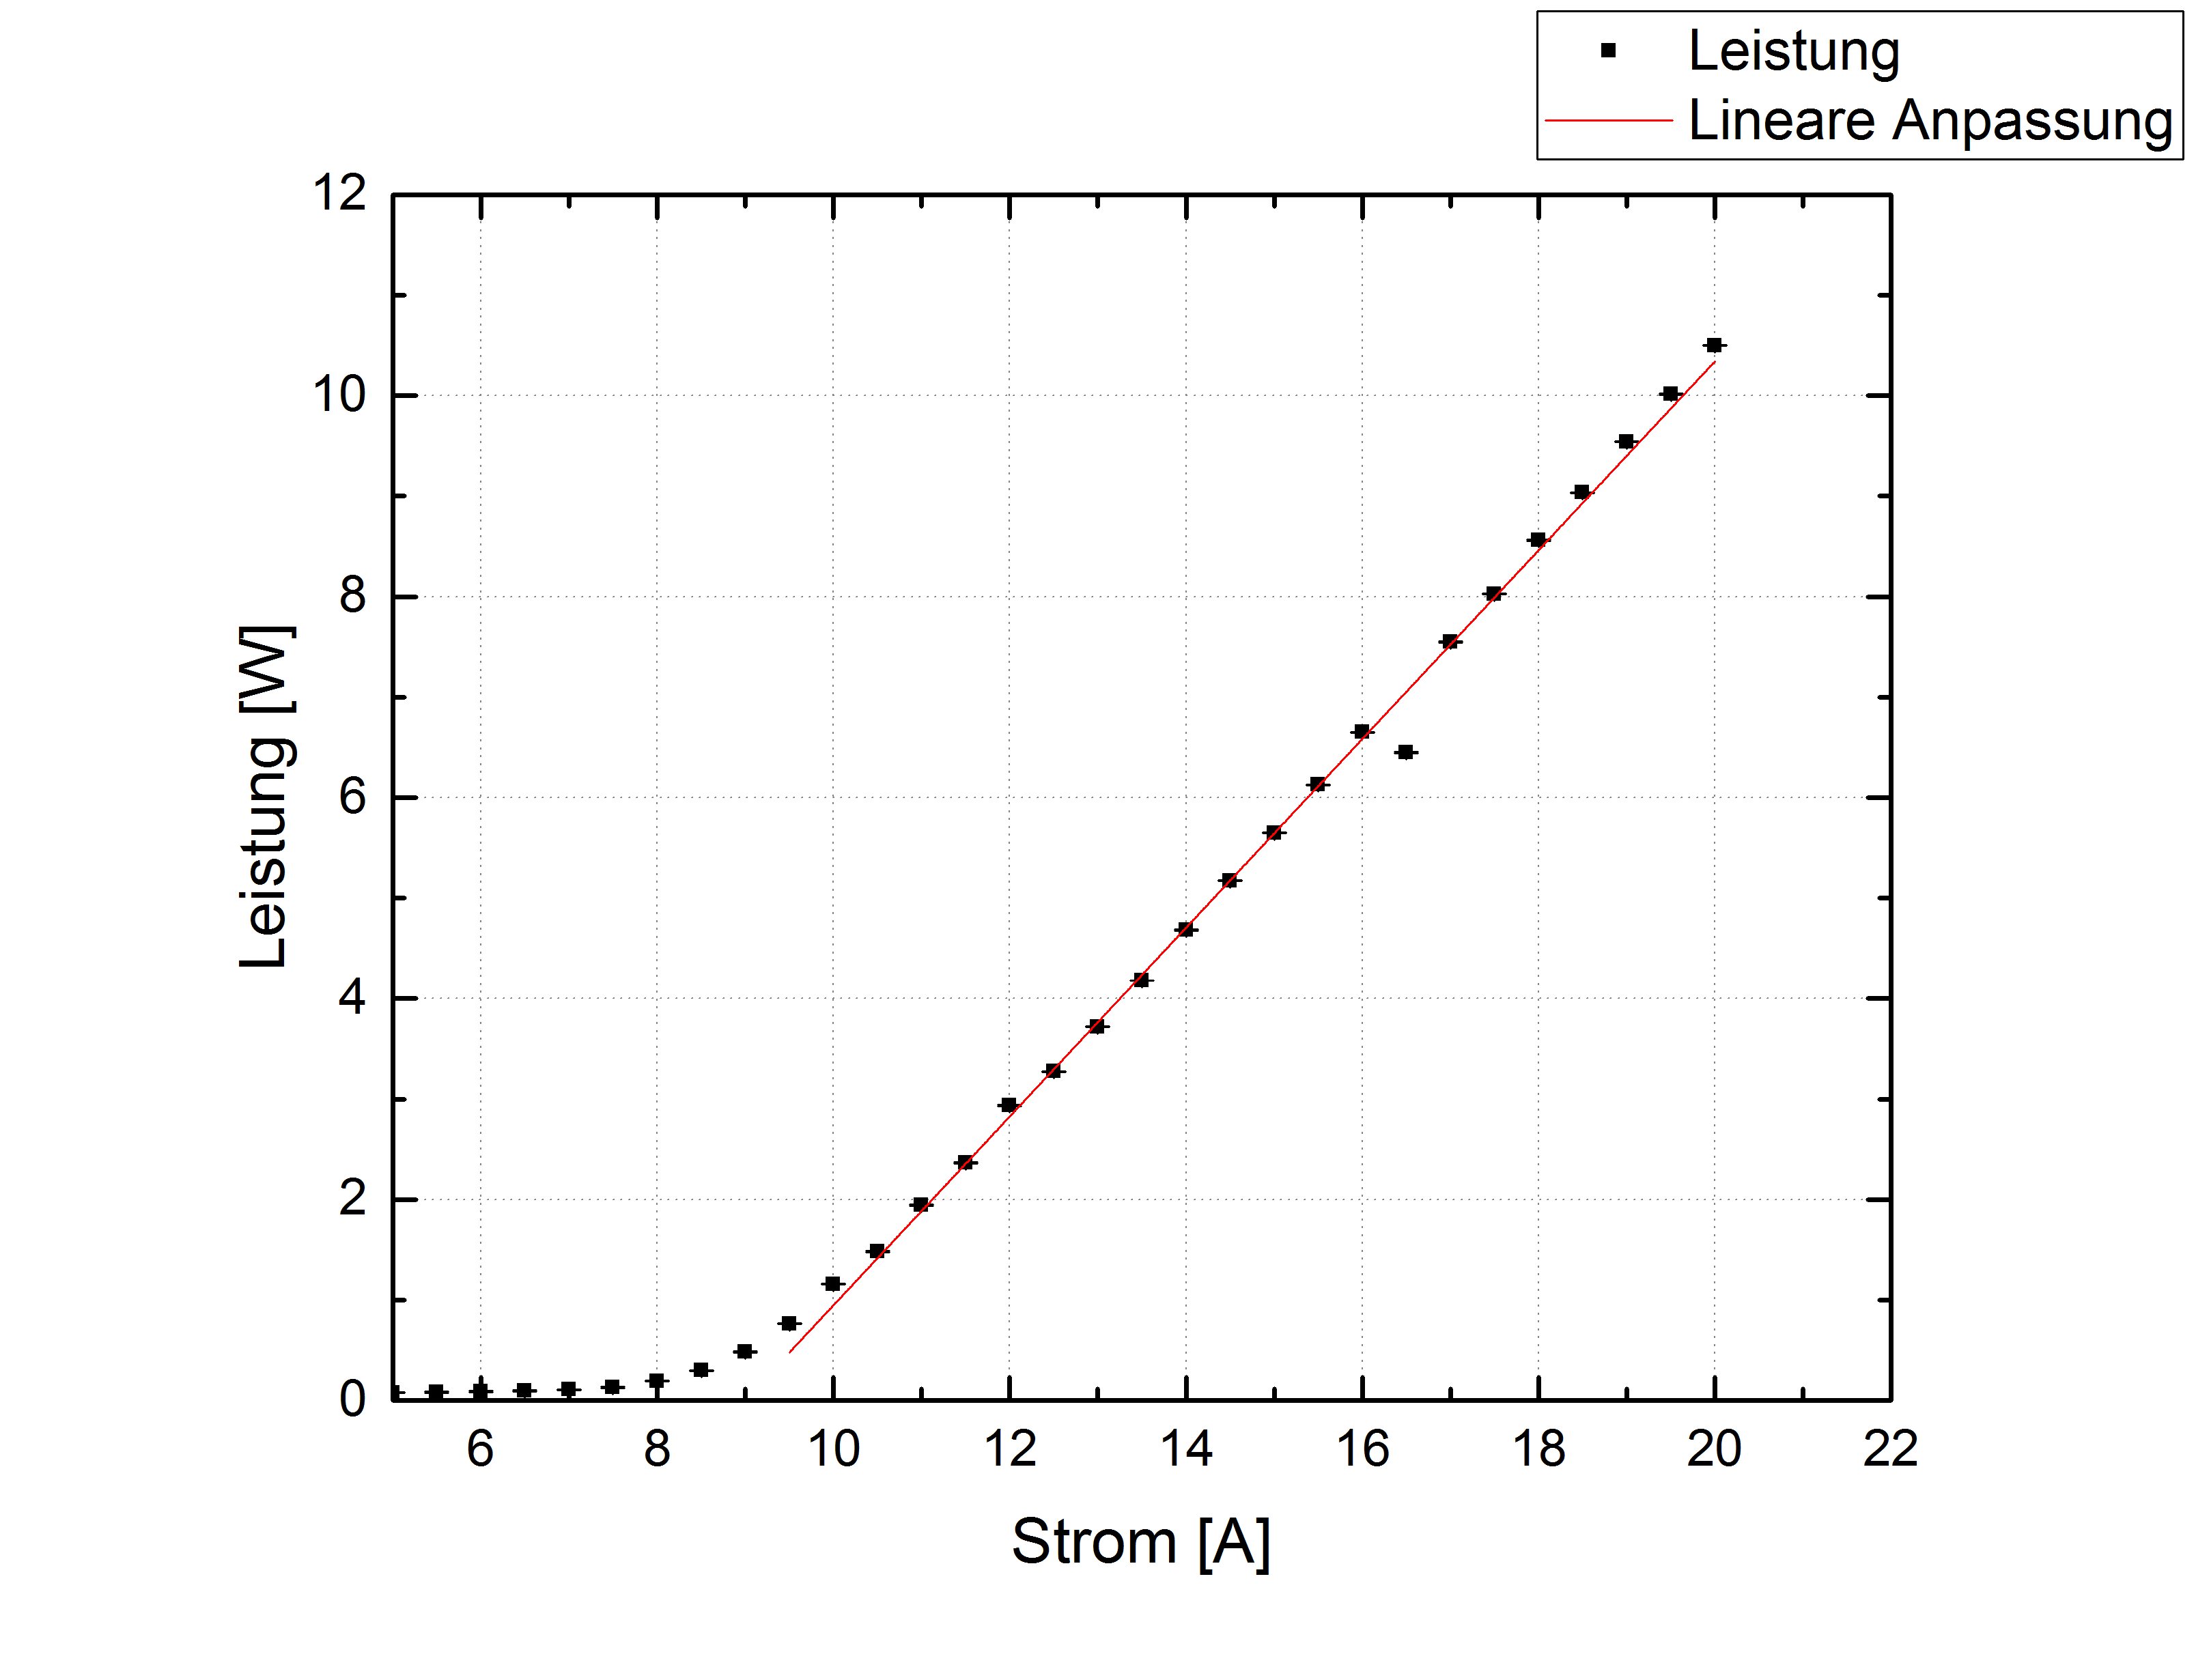
\includegraphics[scale=.5]{Bilder/Pumplaser.png}
		\caption{Kennlinie der Pumpdiode}
		\label{kennpump}
\end{figure}
Der Detektor hat dabei nicht die einfallende Leistung, sondern lediglich die Zahl der einfallenden Photonen gemessen, in Abbildugn \ref{kennpump} wurde jedoch bereits die Umrechnung in Leistung durchgeführt. Dies ist möglich durch die zusätzliche Information, dass die Laserleistung der Diode bei einem Strom von 20A 10.5W beträgt. In diesem Experiment entspricht dies einer Zahl von 1700 womit sich als Umrechnungsfaktor
\begin{equation}
1 \text{ Count}\equiv0.006\text{W}
\end{equation}
Wie leicht zu erkennen ist, gibt es bis zu einem Strom von 8 A keine Nennenswerte Strahlleistung. Dies entpricht nicht ganz der Realität, da aufgrund der hohen Sensivität des Detektors wurden Filter in den Strahlengang gestellt um eine Sättigung zu verhindern. Wie später zu sehen ist, erzeugt die Diode auch in diesem Strombereich, dem Floureszenzbereich, Strahlung, die hier allerdings unterdrückt wird.  \newline
Erhöht man den Strom weiter steigt die Laserleistung langsam bis man ab einem Strom von 9.5A die Lasertätigkeit erreicht hat, in der die Laserleistung der Diode linear mit dem Strom ansteigt. \newline
Der offensichtlich aus der Reihe fallende Wert bei einem Strom von 16.5A beruht wahrscheinlich auf einem falschen Ablesen, er wird aber nicht weiter berücksichtigt, da er die Berechnung weiterer Ergebnisse nicht oder zumindest nicht merklich stört. \newline
Zur Ermittlung des Wirkungsgrades 
\begin{equation}
\eta=\frac{P_{out}}{P_{in}}=\frac{P_{out}}{U\cdot I}\Longrightarrow P_{out}=\eta P_{in}
\label{gl_wirk}
\end{equation}
,also dem Verhältnis zwischen der Leistung die in das System gesteckt wurde und der erhaltenen Leistung wird nur der Bereich der Lasertätigkeit von 9.5A bis 20A betrachtet. Die aufgebrachte Leistung entspricht hier der elektrischen bei einer Spannung von 1.8V und dem jeweils eingestellten Strom. Trägt man diese beiden Leistungen gegeneinander auf so ergibt sich \newline Abbildung \ref{wirkung}
\begin{figure}[H]
	\begin{center}
		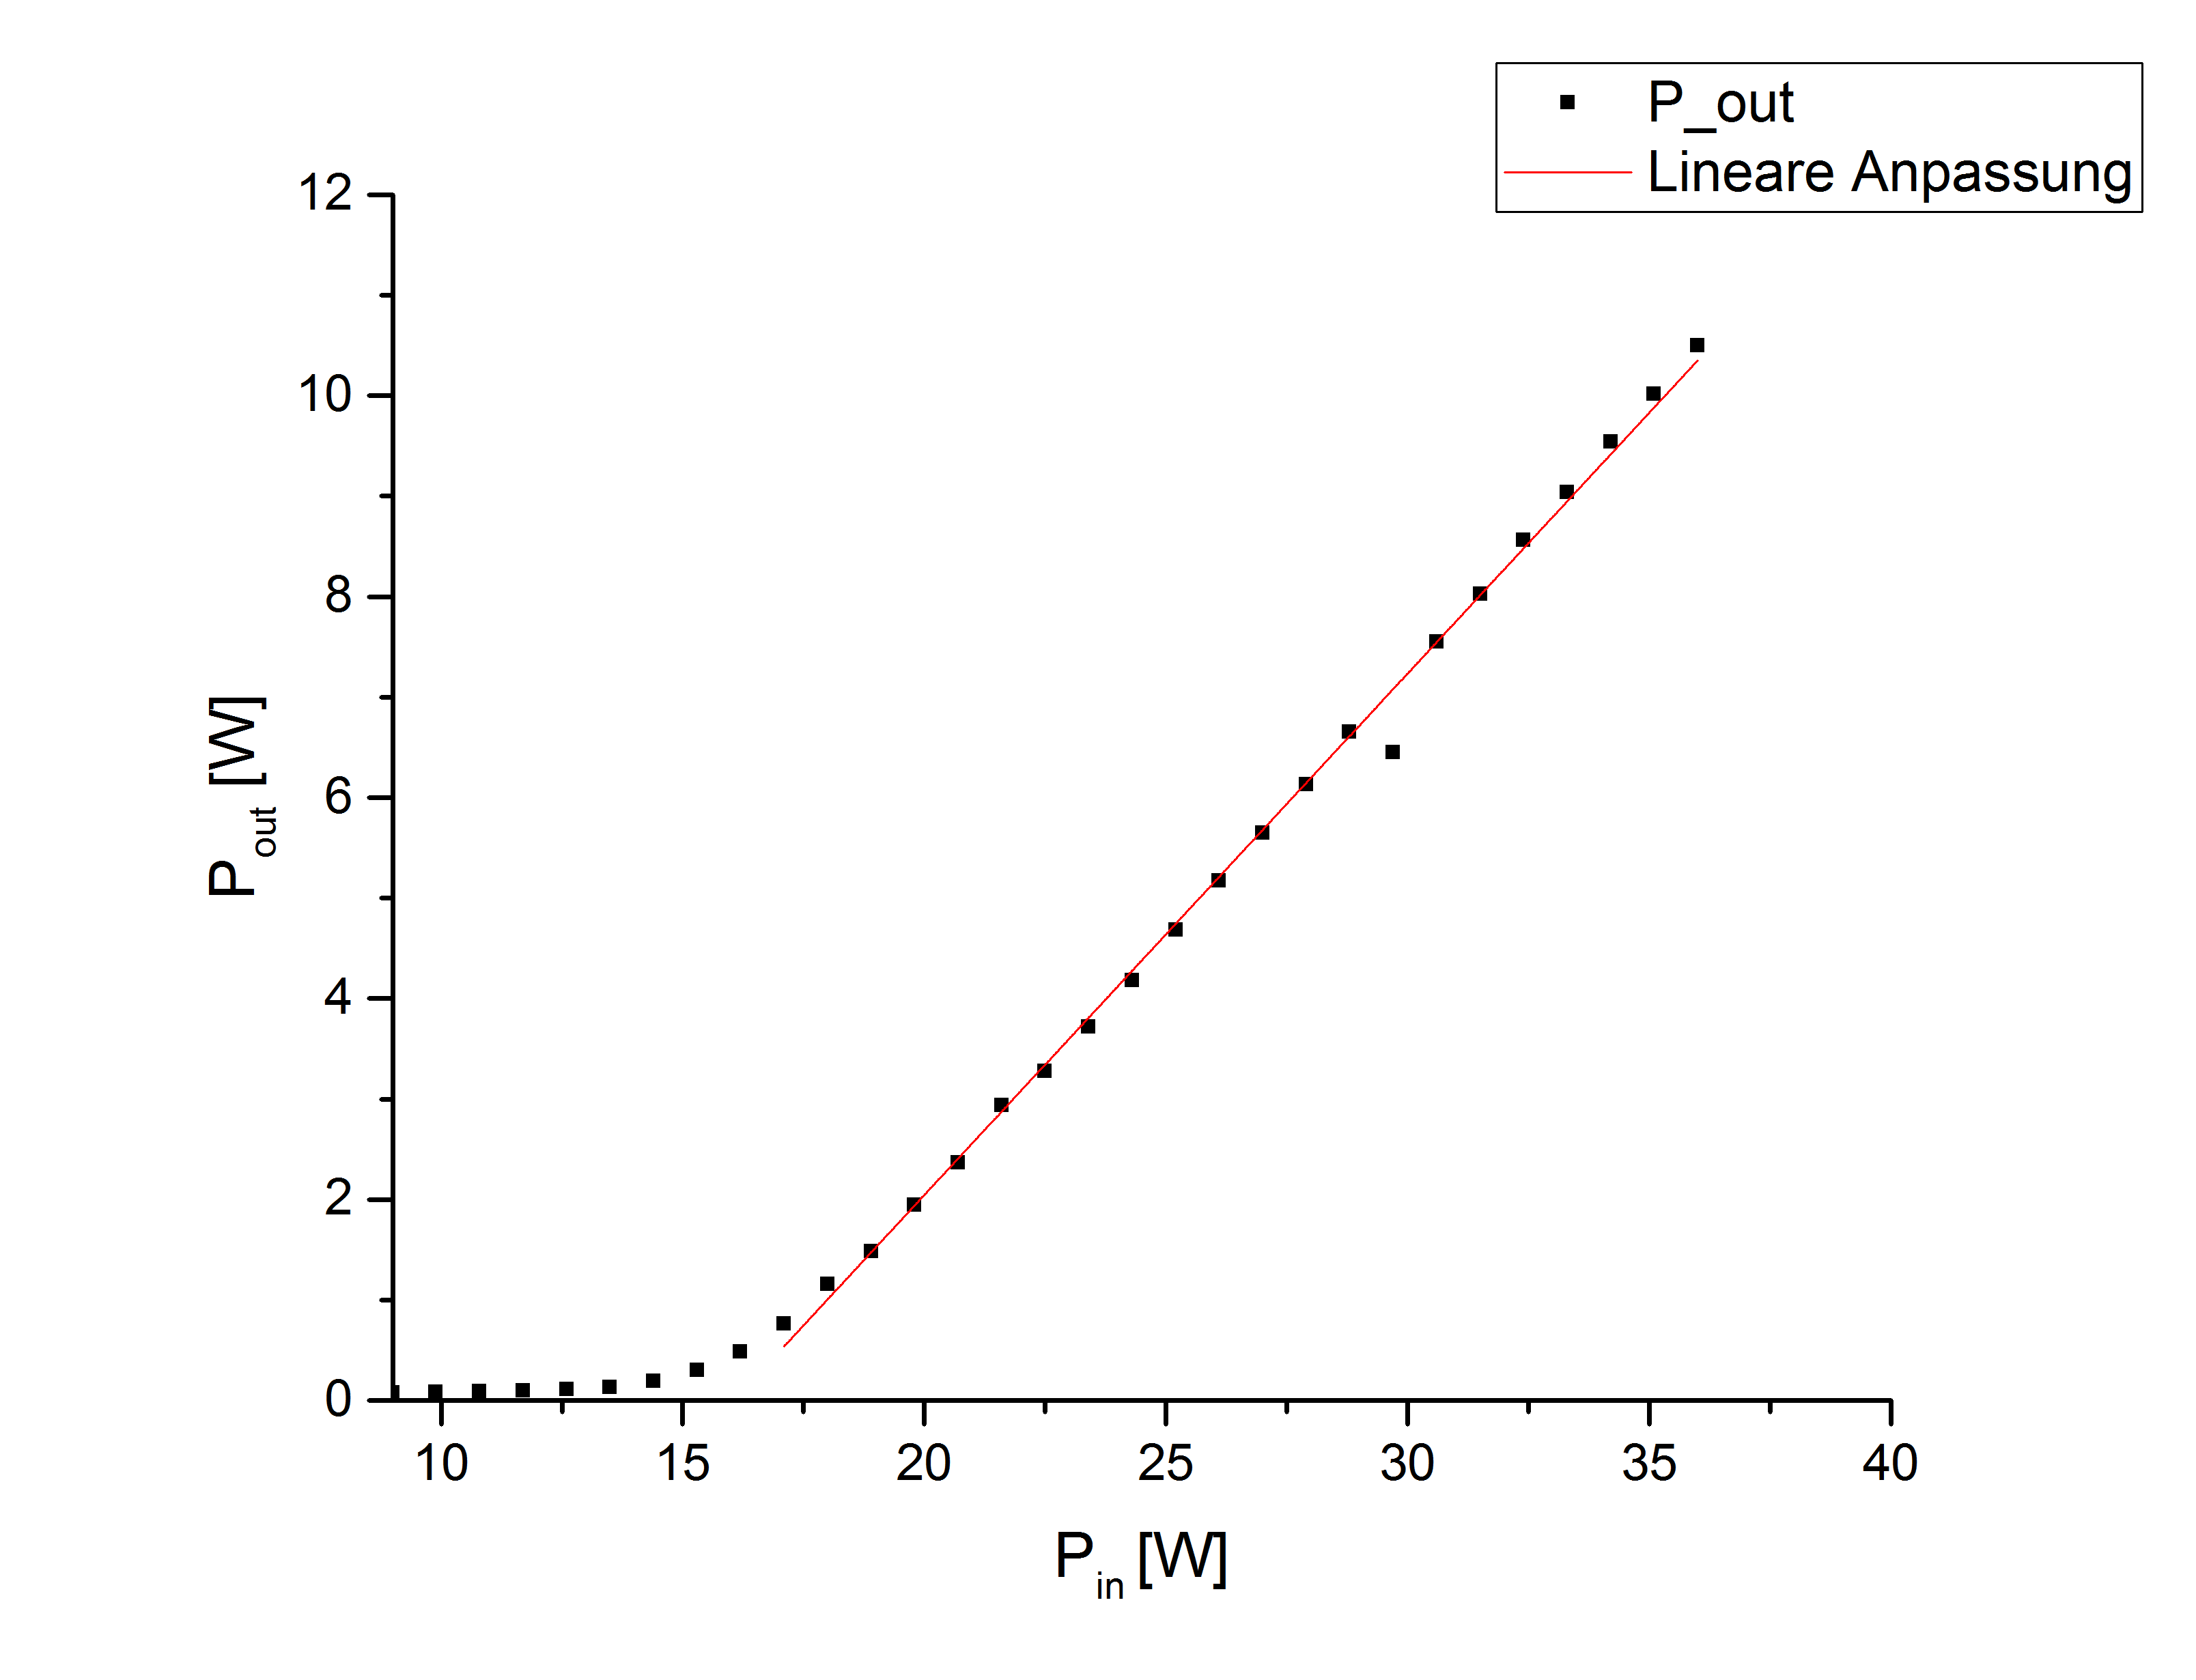
\includegraphics[scale=.5]{Bilder/Wirkungsgrad.png}
		\caption{Wirkungsgrad der Pumpdiode}
		\label{wirkung}
	\end{center}
\end{figure}
Wie sich aus Gleichung (\ref{gl_wirk}) leicht ablesen lässt, entspricht der Wirkungsgrad der Diode genau der Steigung der Ausgleichsgeraen und es ergibt sich
\begin{equation}
\eta=0.519\pm0.006=(51.9\pm0.6)\%
\end{equation}
\subsection{"`Slope efficiency"' des Nd:YLF-Lasers}
Die sogenannten slope efficiency eines Lasers ist das Verhältnis aus Pumpleistung die dem System zugeführt wird und der eigentlichen Laserleistung oberhalb der Laserschwelle, gibt also in gewissem Sinne den Wirkungsgrad des Lasers wieder. Da aufgrund des experimentellen Aufbaus schon vor erreichen des eigentlichen Laserkörpers 50\% des Lichtes aus der Pumpdiode ausgekoppelt werden, müssen die im vorigen Versuch ermittelten Pumpleistungen für die Berechnung der slope efficiency halbiert werden und man erhält Abbildung \ref{slope}.
\begin{figure}[H]
	\begin{center}
		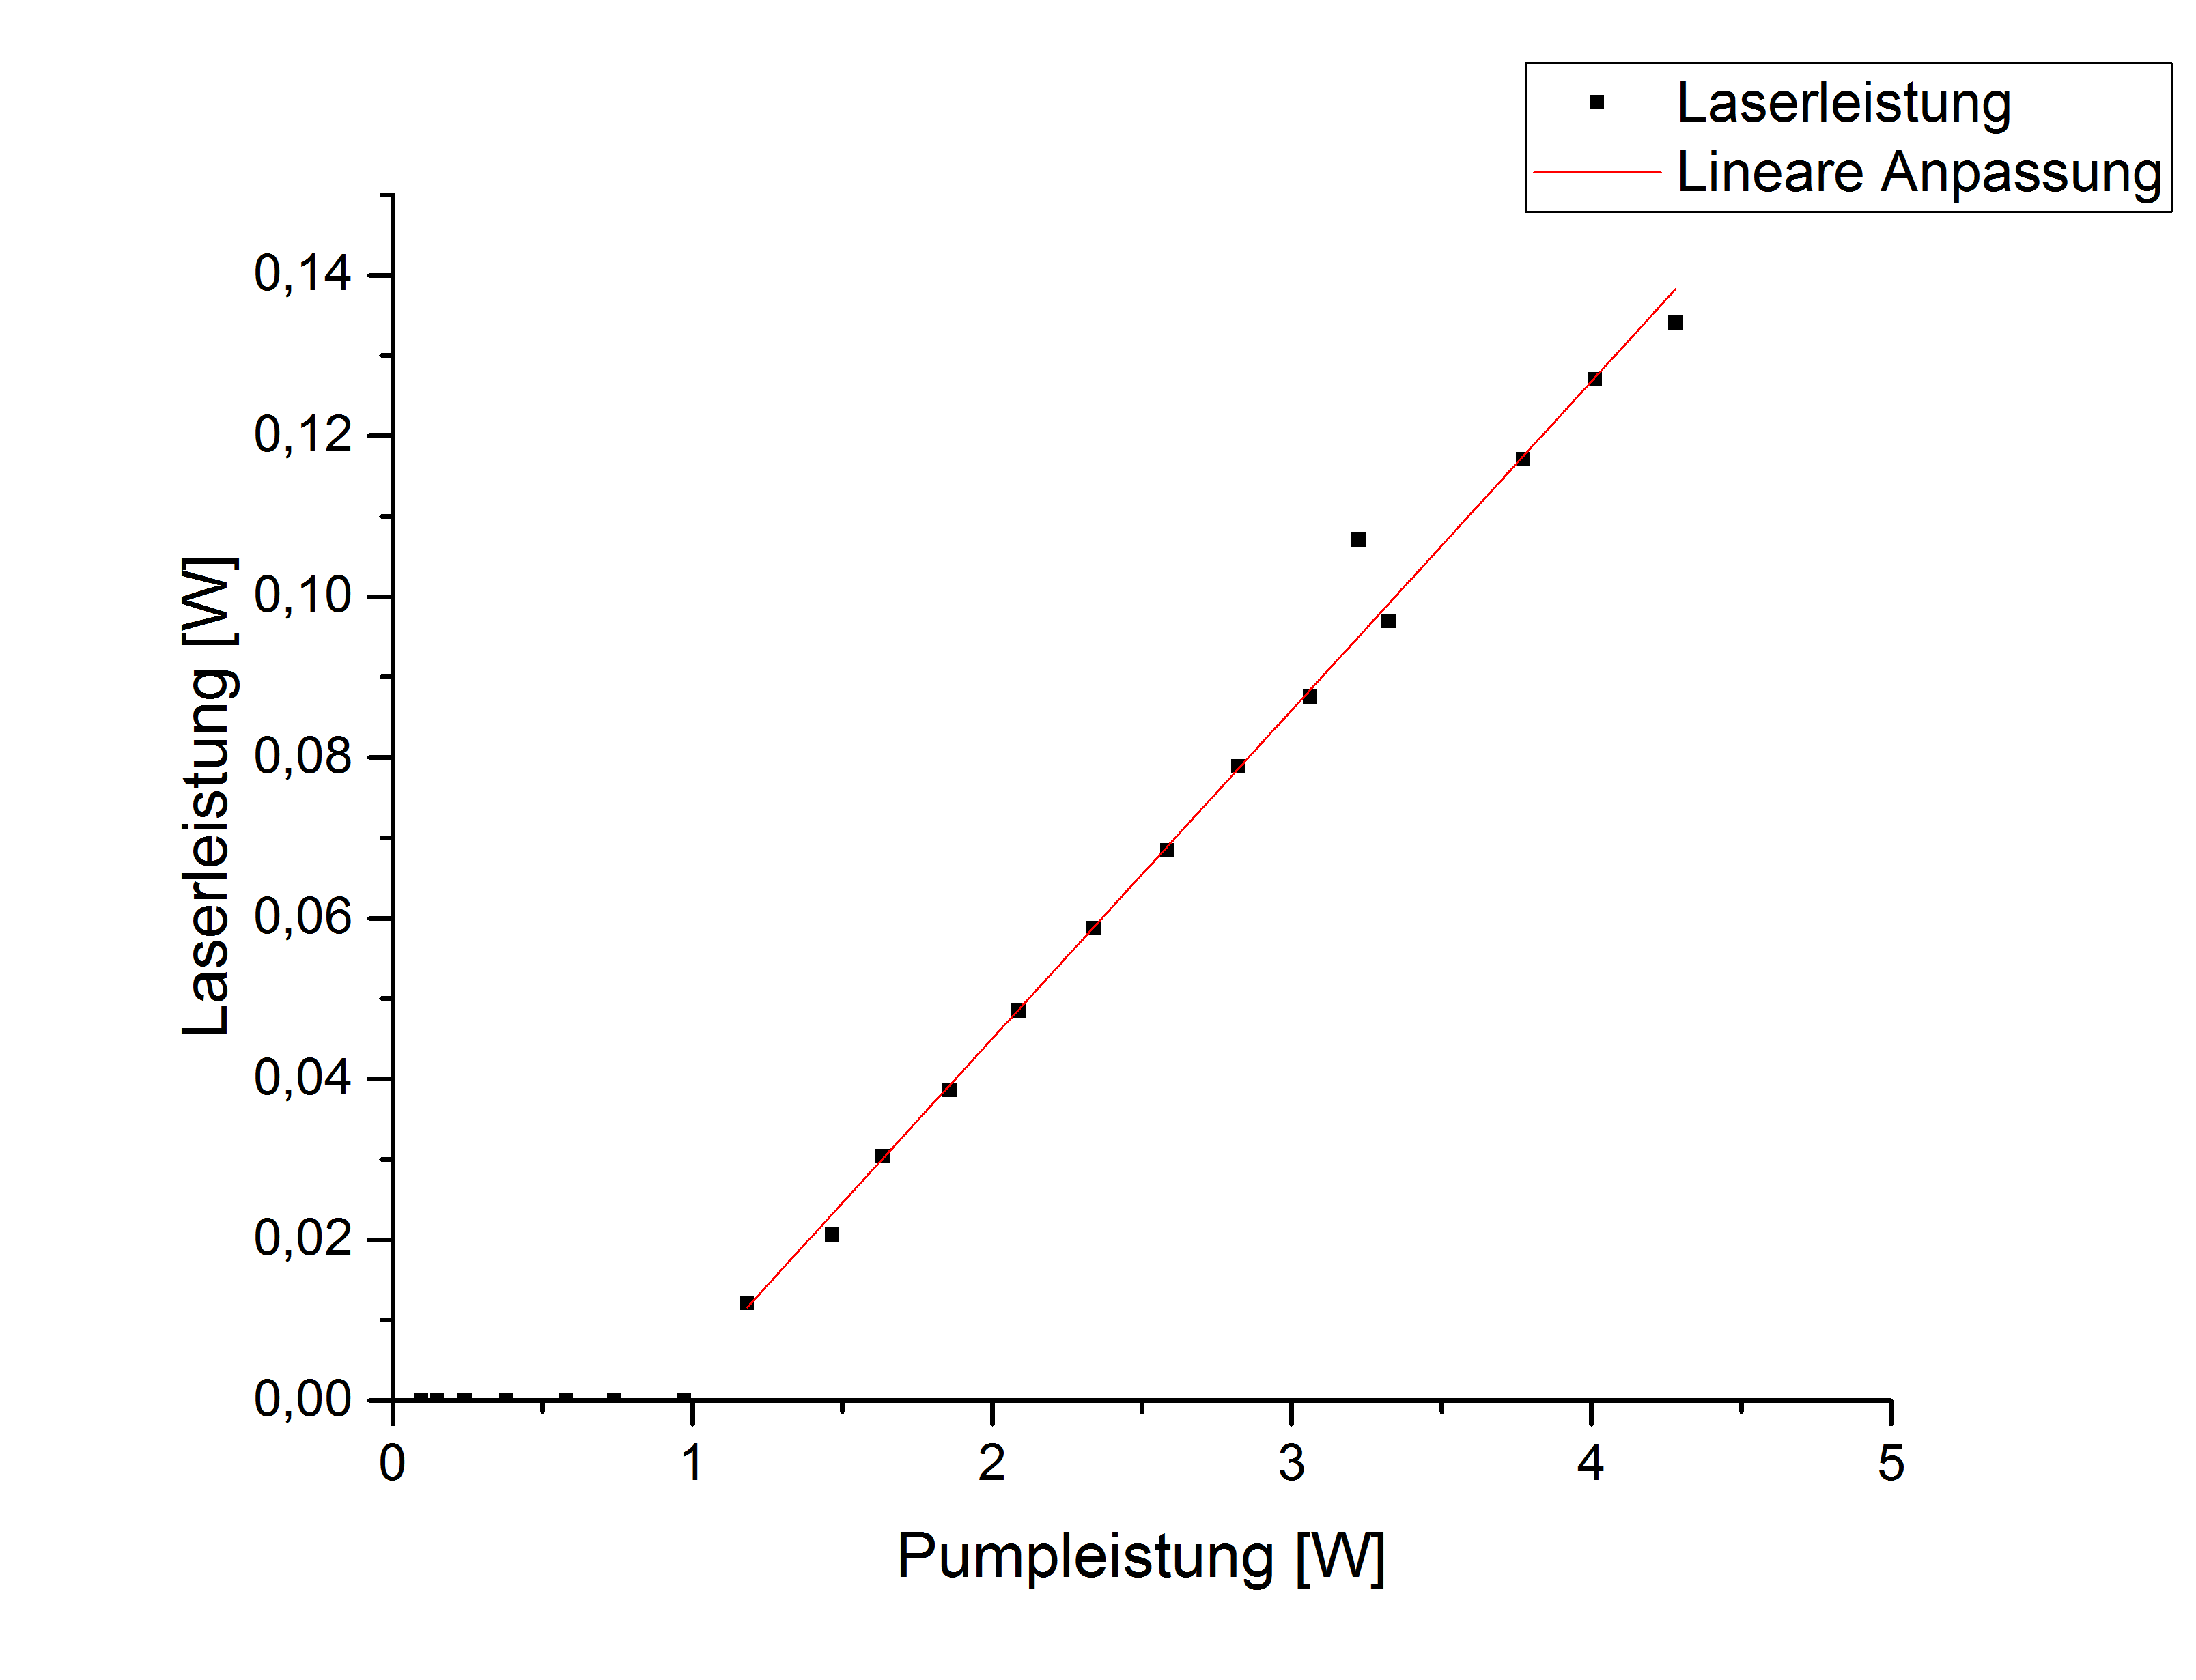
\includegraphics[scale=.5]{Bilder/slope.png}
		\caption{slope efficiency des Nd:YLF-Lasers}
		\label{slope}
	\end{center}
\end{figure}
Man erkennt auch hier einen stark linearen Zusammenhang zwischen eingehender und Pumpleistung, die Steigung der Gerade gibt dabei die slope efficency $\sigma$ an und es ergibt sich
\begin{equation}
\sigma=0.041\pm0.001=(4.1\pm0.1)\%
\end{equation}
\subsection{Autokorellationsmessung}
Um die Impulsdauer des Lasespulses zu bestimmen wird eine Autokorellationsmessung genutzt. Hier wird der Laserpuls in zwei separate Teile aufgespalten und durch zwei unterschiedlich lange Wegstrecken geschickt. Nach dem Durchqueren dieser Verzögerungsstrecken überlagern sich beide Impulsanteile in einem nicht-linearen Kristall zu einer Oberwelle, deren Intesität in Abhängigkeit von der Verzögerungszeit t$_D$ der beiden Impulsanteile zueinander gemessen wird. 
\begin{figure}[H]
	\begin{center}
		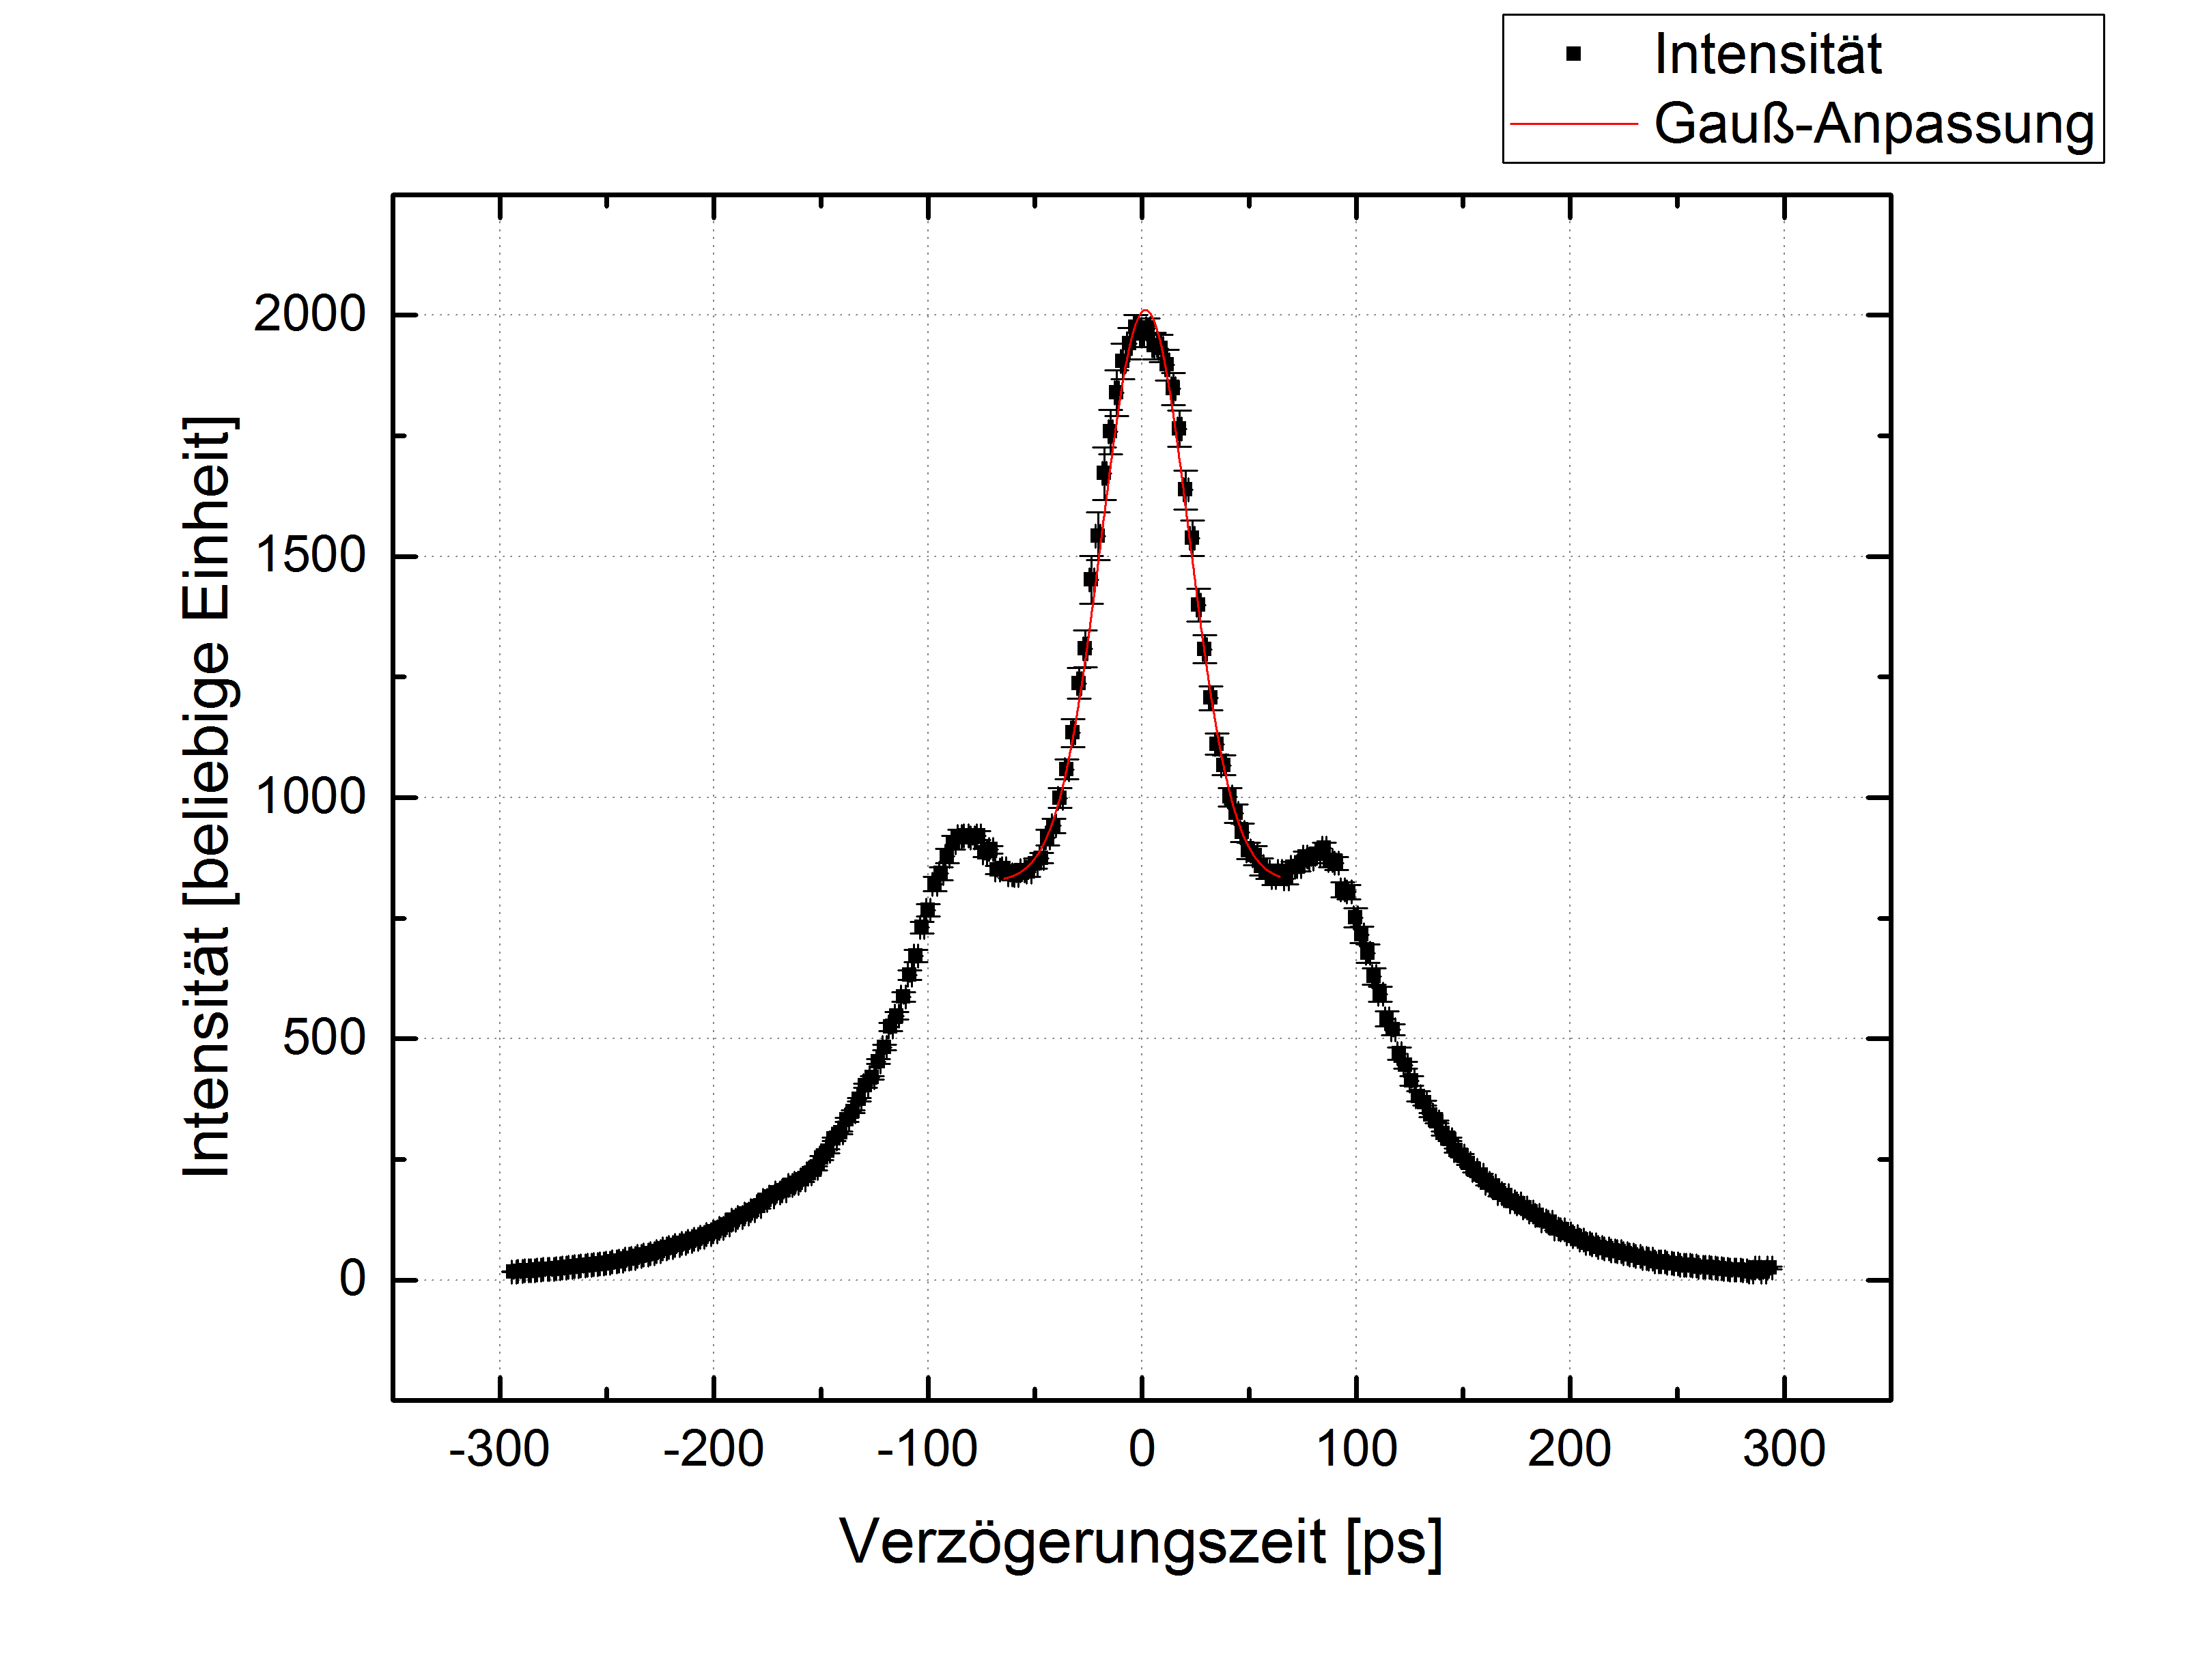
\includegraphics[scale=.5]{Bilder/Autokorr1.png}
		\caption{Autokorellationsfunktion in Abhängigkeit von der Verzögerungszeit}
		\label{aut1}
	\end{center}
\end{figure}
Wie in Abbildung \ref{aut1} zu sehen ist, tauchen neben dem relevanten Maximum um t$_D$=0 zwei weitere Maxima auf, die aufgrund der Symmetrie der Autokorellationsfunktion symmetrisch um das Hauptmaximum angeordnet sind. Eine Erklärung hierfür steht noch aus und auch vorhergehende Bemühungen der Verantwortlichen des Versuchs diese Nebenmaxima zu eliminieren scheiterten, weshalb sich im Folgenden nur mit dem Hauptmaximum um t$_D$=0 befasst wird, welches in Abbildung \ref{aut2} genauer gezeigt ist.
\begin{figure}[H]
	\begin{center}
		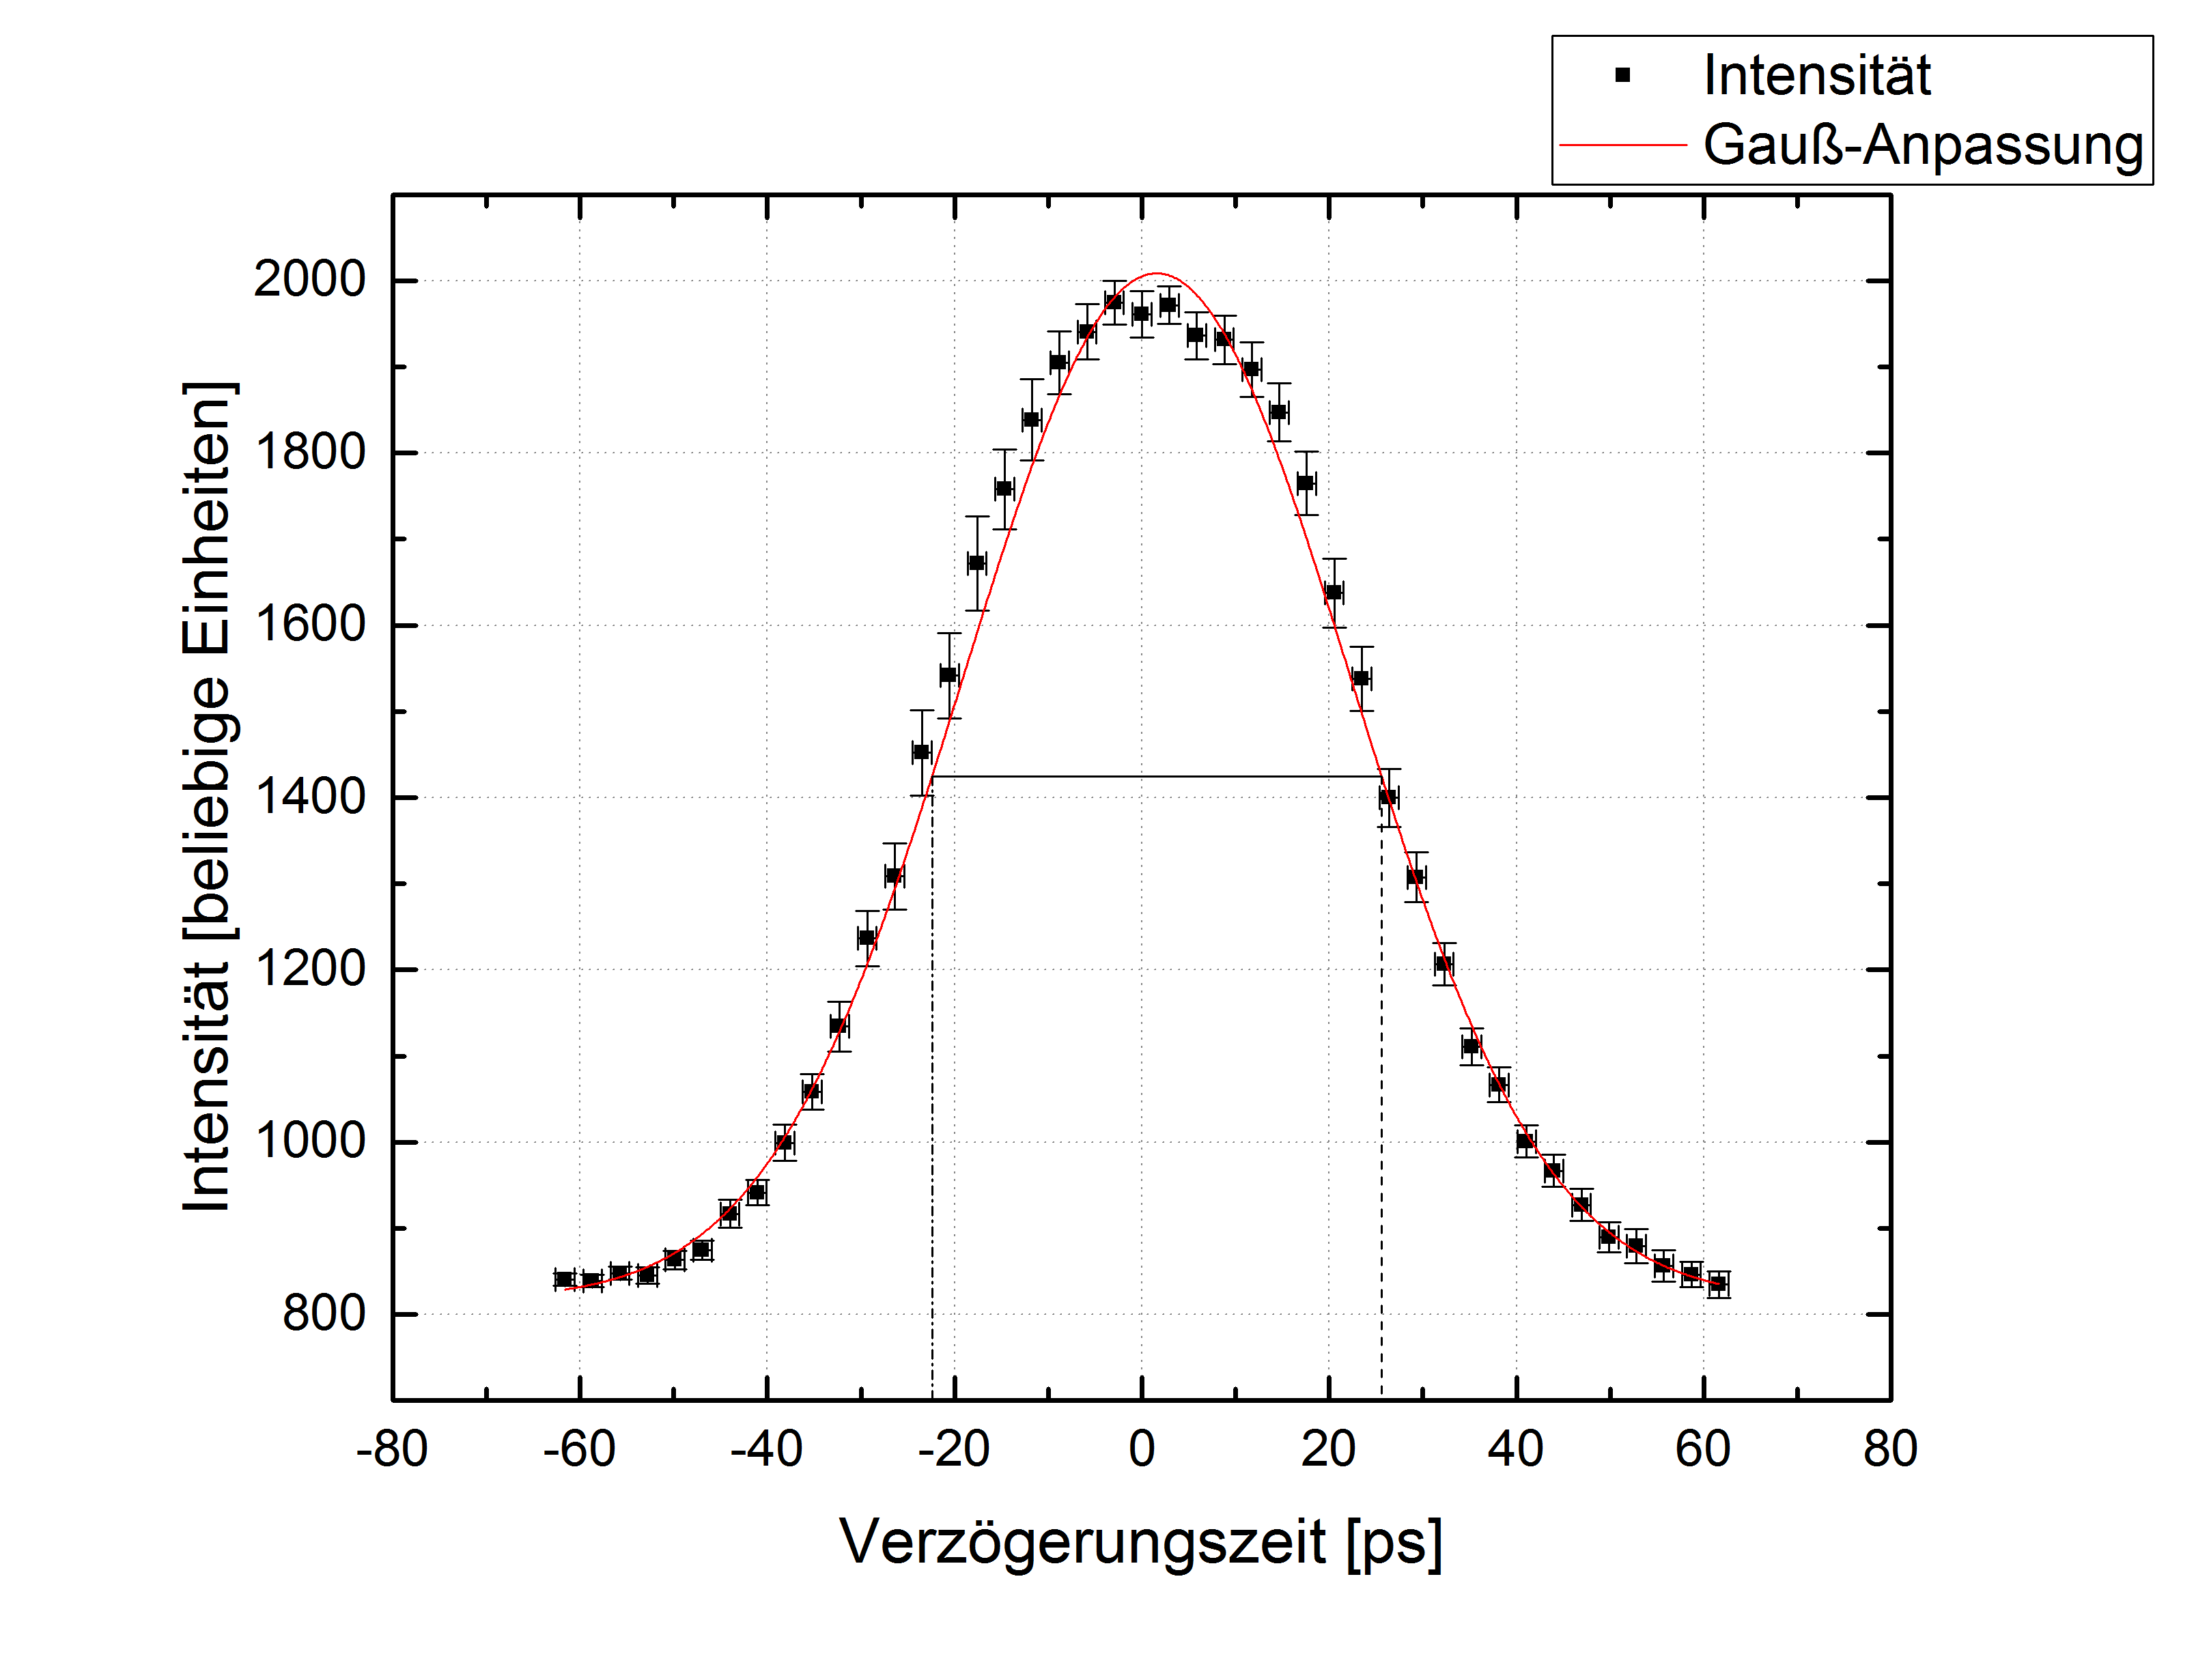
\includegraphics[scale=.5]{Bilder/Autokorr2.png}
		\caption{Hauptmaximum der Autokorrelationsfunktion}
		\label{aut2}
	\end{center}
\end{figure}
Es ist zu erkennen, dass die Intensität gaußförmig verteilt ist, was für einen modengekoppelten Puls der Form
\begin{equation*}
I(t)=I_0\cdot e^{-At}
\end{equation*}
wie er hier verwendet wurde, wobei A=$\frac{4\ln2}{\tau}$ mit $\tau$ der Halbwertsbreite des Pulses, zu erwarten war, da die Autokorrelationsfunktion sich so zu 
\begin{equation*}
W(t_D)\propto\int_{-\infty}^{\infty}e^{-A(t-t_D)^2}\:e^{-At^2}\:dt\propto e^{-\frac{A}{2}t_D^2}
\end{equation*}
Es ergibt sich also eine Gauß-Kurve mit einer Halbwertsbreite $\tau'$, die in folgendem Zusammenhang mit der Halbwertsbreite des Pulses steht.
\begin{equation}
\tau'=\sqrt{2}\:\tau
\end{equation}
Eine Auswertung der gemessenen Autokorellationsfunktion ergibt 
\begin{equation}
\tau'=(48.677\pm0.538)\text{ps}\Longrightarrow\tau=(34.420\pm0.380)\text{ps}
\end{equation}
\subsection{Winkelabhängigkeit der Intensität der ersten Oberwelle}
Bei der Überlagerung der einzelnen Impulsanteile nach Durchlauf der Verzögerungsstrecken kommt es jedoch zu einem Problem. Die erzeugte Oberwelle und die Fundamentale Welle stehen im Allgemeinenen nicht in einer festen Phasenbeziehung zueinander, da $\triangle k=2k_\omega-k_{2\omega}\neq0$, anstatt einer einer kontinuirlichen Verstärkung des Signals kommt es so zu sich periodisch wiederholender konstruktiver und destruktiver Interferenz. Um dieses Problem zu beheben wählt man als Überlagerungsmedium eine nicht-lineare Substanz, in diesem Fall Beta-Bariumoxid, welche für verschieden Polarisationsrichtungen des einfallenden Feldes jeweils verschiedene Brechungsindizes aufweist. \newline
Ist der Strahl senkrecht zur optischen Achse des Kristalls polarisiert so erfährt er den ordentlichen Brechungsindex n$_o$, ist er jedoch parallel dazu polarisiert, so merkt er den außerordentlichen Brechungsindex n$_a$. \newline
Wählt man nun die Oberwelle als außerordentlichen und die Fundamentale als ordentlichen Strahl, so lässt sich der Brechungsindex für die Außerordentliche in Abhängigkeit des Winkels zwischen Polarisation und optischer Achse $\theta$ in einem Bereich n$_a\leq$ n$\leq$ n$_o$ nach (\ref{pol}) beliebig einstellen.
\begin{equation}
\frac{1}{n(\theta)^2}=\frac{1}{n_a^2}+\left(\frac{1}{n_o^2}-\frac{1}{n_a^1}\right)\cos^2\theta
\label{pol}
\end{equation}
Um nun eine Phasenanpassung zwischen der Fundamentalen mit der Frequenz $\omega$ und der Oberwelle mit Frequenz 2$\omega$ zu erreichen, also für $\triangle k=0$ muss
\begin{equation}
n(\theta)=n_\omega=n_{o,\omega}
\end{equation}
erfüllt sein. Setzt man dies in \ref{pol} ein, löst nach $\theta$ auf und setzt die passenden Werte für die Brechungsindices ein, so ergibt sich ein Phasenanpassungswinkel von
\begin{equation}
\theta=0.40=21.10^\circ
\end{equation}
Dies entspricht allerdings nur der Ausrichtung des einfallenden Pulses zu der optischen Achse, nicht zu der Kristalloberfläche. Die Abhängigkeit Intensität von der Ausrichtung des Kristalls ist in Abbildung \ref{winkel} gezeigt.
\begin{figure}[H]
	\begin{center}
		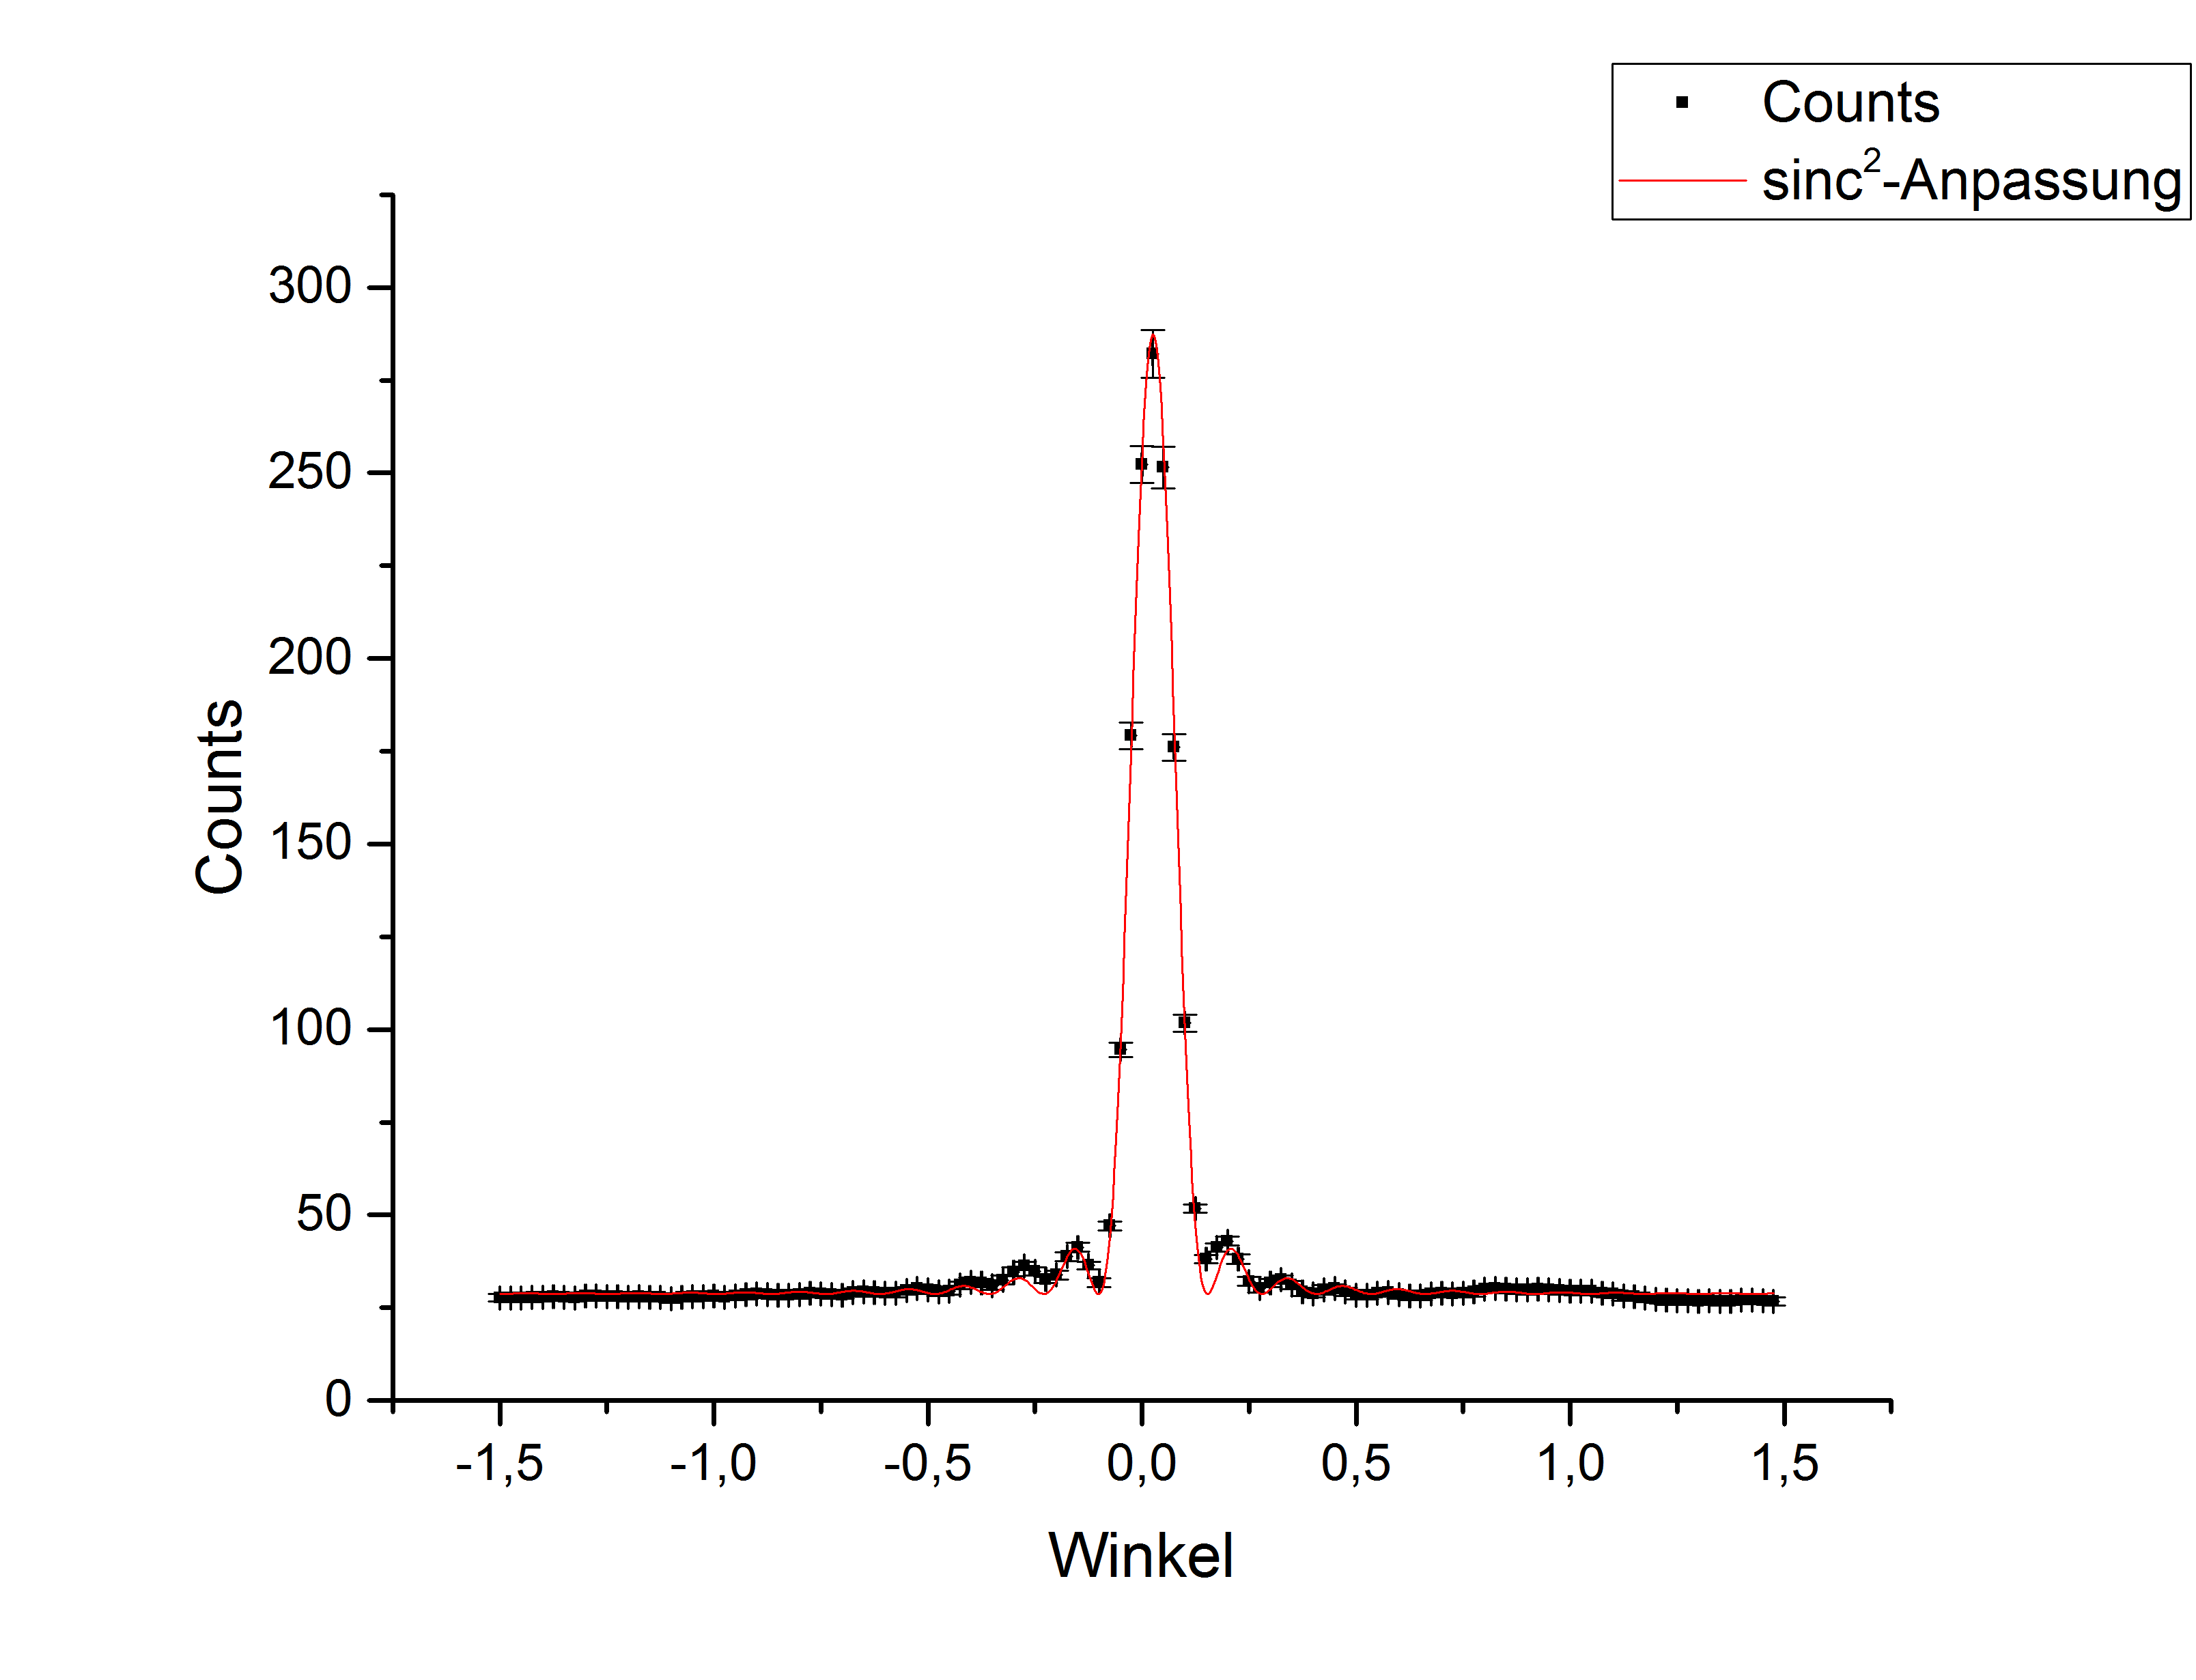
\includegraphics[scale=.5]{Bilder/Winkel.png}
		\caption{Winkelabhängigkeit der Intensität der Oberwelle}
		\label{winkel}
	\end{center}
\end{figure}
Nach 
\begin{equation}
I\propto \frac{\sin^2\left(\triangle k \frac{l}{2}\right)}{\left(\triangle k \frac{l}{2}\right)^2}=\text{sinc}^2\left(\triangle k \frac{l}{2}\right)
\label{sinc}
\end{equation}
folgt die Intensität einer sinc$^2$-Kurve, was aus Abbildung \ref{winkel} ersichtlich ist. Die Funktion, die zum Anpassen genutzt wurde lautet dabei
\begin{equation}
I=258.684\cdot\text{sinc}^2\left(24.657\cdot\theta-0.639\right)+28.726
\end{equation}
Die Intensität wird dabei in Einheiten von Counts, also der Anzahl der einfallenden Photonen angegeben und ist somit einheitenlos. \newline
Um nun die Maxima beziehungsweise Minima der Intensität zu finden müssen die Winkel ermittelt werden, bei denen das Argument der sinc-Funktion gleich $\pi$ oder $\frac{\pi}{2}$ sind. Es ergibt sich also
\begin{eqnarray}
24.657\cdot\theta-0.639\overset{!}{=}\pi\Longrightarrow\theta_1=0.153\\
24.657\cdot\theta-0.639\overset{!}{=}\frac{\pi}{2}\Longrightarrow\theta_2=0.090
\end{eqnarray}
Somit ergibt sich eine effetkive Weglänge l$_{eff}$ der Oberwelle durch den Kristall von 
\begin{equation}
l_{eff}=\frac{l}{\cos\alpha}=\frac{l}{\cos\left(\arcsin\left(\frac{\sin\theta}{n_{a,2\omega}}\right)\right)}=\left\{\begin{array}{ll} 4.019\text{ mm},  \;\; &\theta=\pi\\\\
4.007\text{ mm}, &\theta = \frac{\pi}{2}\end{array}\right.
\end{equation}
Der Ausdruck für den Winkel $\alpha$ in dem Kristall ergibt sich aus dem Snelliusschem Brechungsgesetz.\newline
Womit sich eine Wellenvektorfehlapassung $\triangle k$ von 
\begin{equation}
\triangle k\cdot \frac{l_{eff}}{2}=\left\{\begin{array}{ll} \pi \Longrightarrow \triangle k=1.563\frac{1}{\text{mm}} \\\\
\frac{\pi}{2}\Longrightarrow \triangle k=1.568\frac{1}{\text{mm}}  \end{array}\right.
\end{equation}
\subsection{Intensitätsabhängigkeit der Intensität der ersten Oberwelle}
Die Intensität hängt jedoch nicht nur von der Ausrichtung des Kristalls aus, sondern natürlicherweise auch von der Ausgangintensität des Lasers aus. Im Folgenden wurde also die die Laserintensität vor Aufteilung des Pulses durch ein $\frac{\lambda}{2}$-Plättchen moduliert. \newline
Naiv wäre eine lineare Abhängigkeit zwischen Laserintensität und der Intensität der Oberwelle zu erwarten. Berechnungen zeigen allerdings, dass neben (\ref{sinc}) auch
\begin{equation}
I_{2\omega}\propto I_\omega^2
\end{equation}
gilt, es also ein quadratischer Zusammenhang gilt, was auch die graphische Auswertung zeigt. Um dies zu zeigen wurden die Intensitäten des Lasers und der Oberwelle gegeneinander aufgetragen und ein Polynom 9. Grades als Ausgleichsfunktion genutzt, was in Abbildung \ref{pol9} zu sehen ist.
\begin{figure}[H]
	\begin{center}
		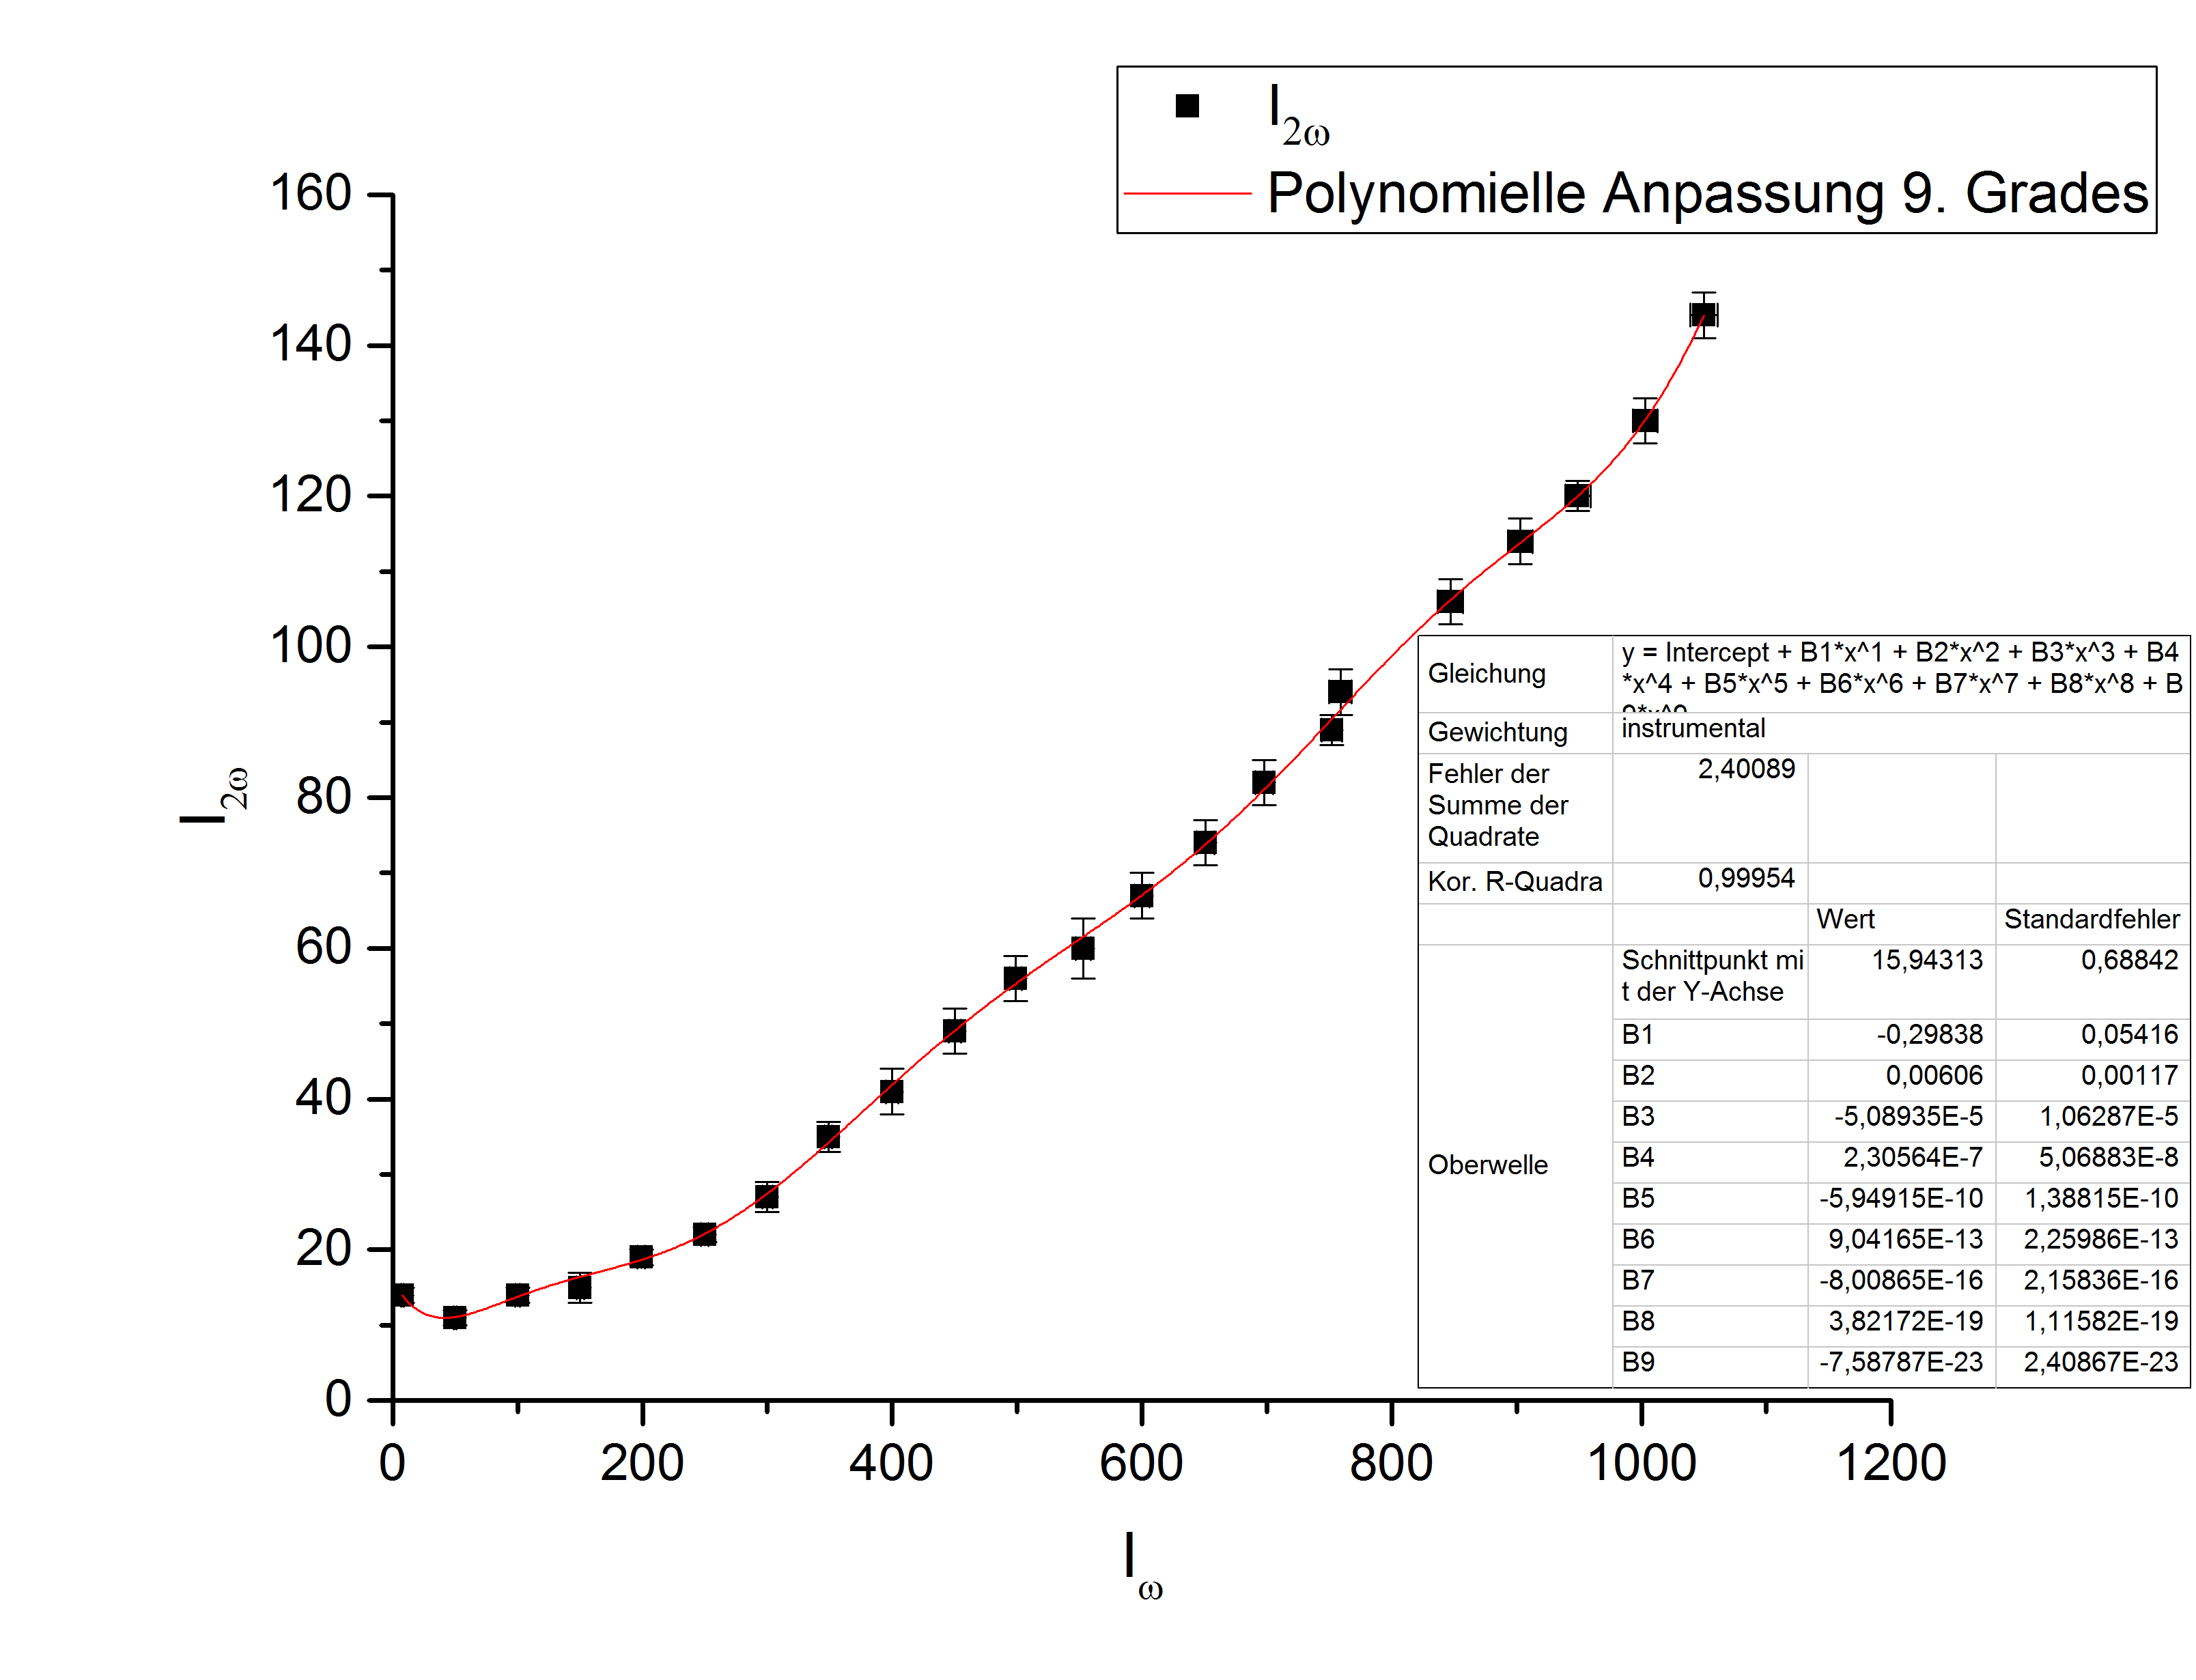
\includegraphics[scale=.5]{Bilder/IntPol9.png}
		\caption{Anpassung der Intensitätsabhängigkeit durch ein Polynom 9. Grades}
		\label{pol9}
	\end{center}
\end{figure}
Man erkennt, dass das Polynom zwar sämtliche Messpunkte jeweils genau trifft, betrachtet man jedoch die Vorfaktoren des Polynoms in Abbildung \ref{pol9}, so ist leicht einzusehen, dass diese für Potenzen > 2 so verschwindend klein sind, dass sie zu vernachlässigen sind. Man erhält also ein Polynom 2. Grades als Ausgleich, was auch die Rechnung ergeben hat. Abbildung \ref{pol2} zeigt genau dieses Verhalten
\begin{figure}[H]
	\begin{center}
		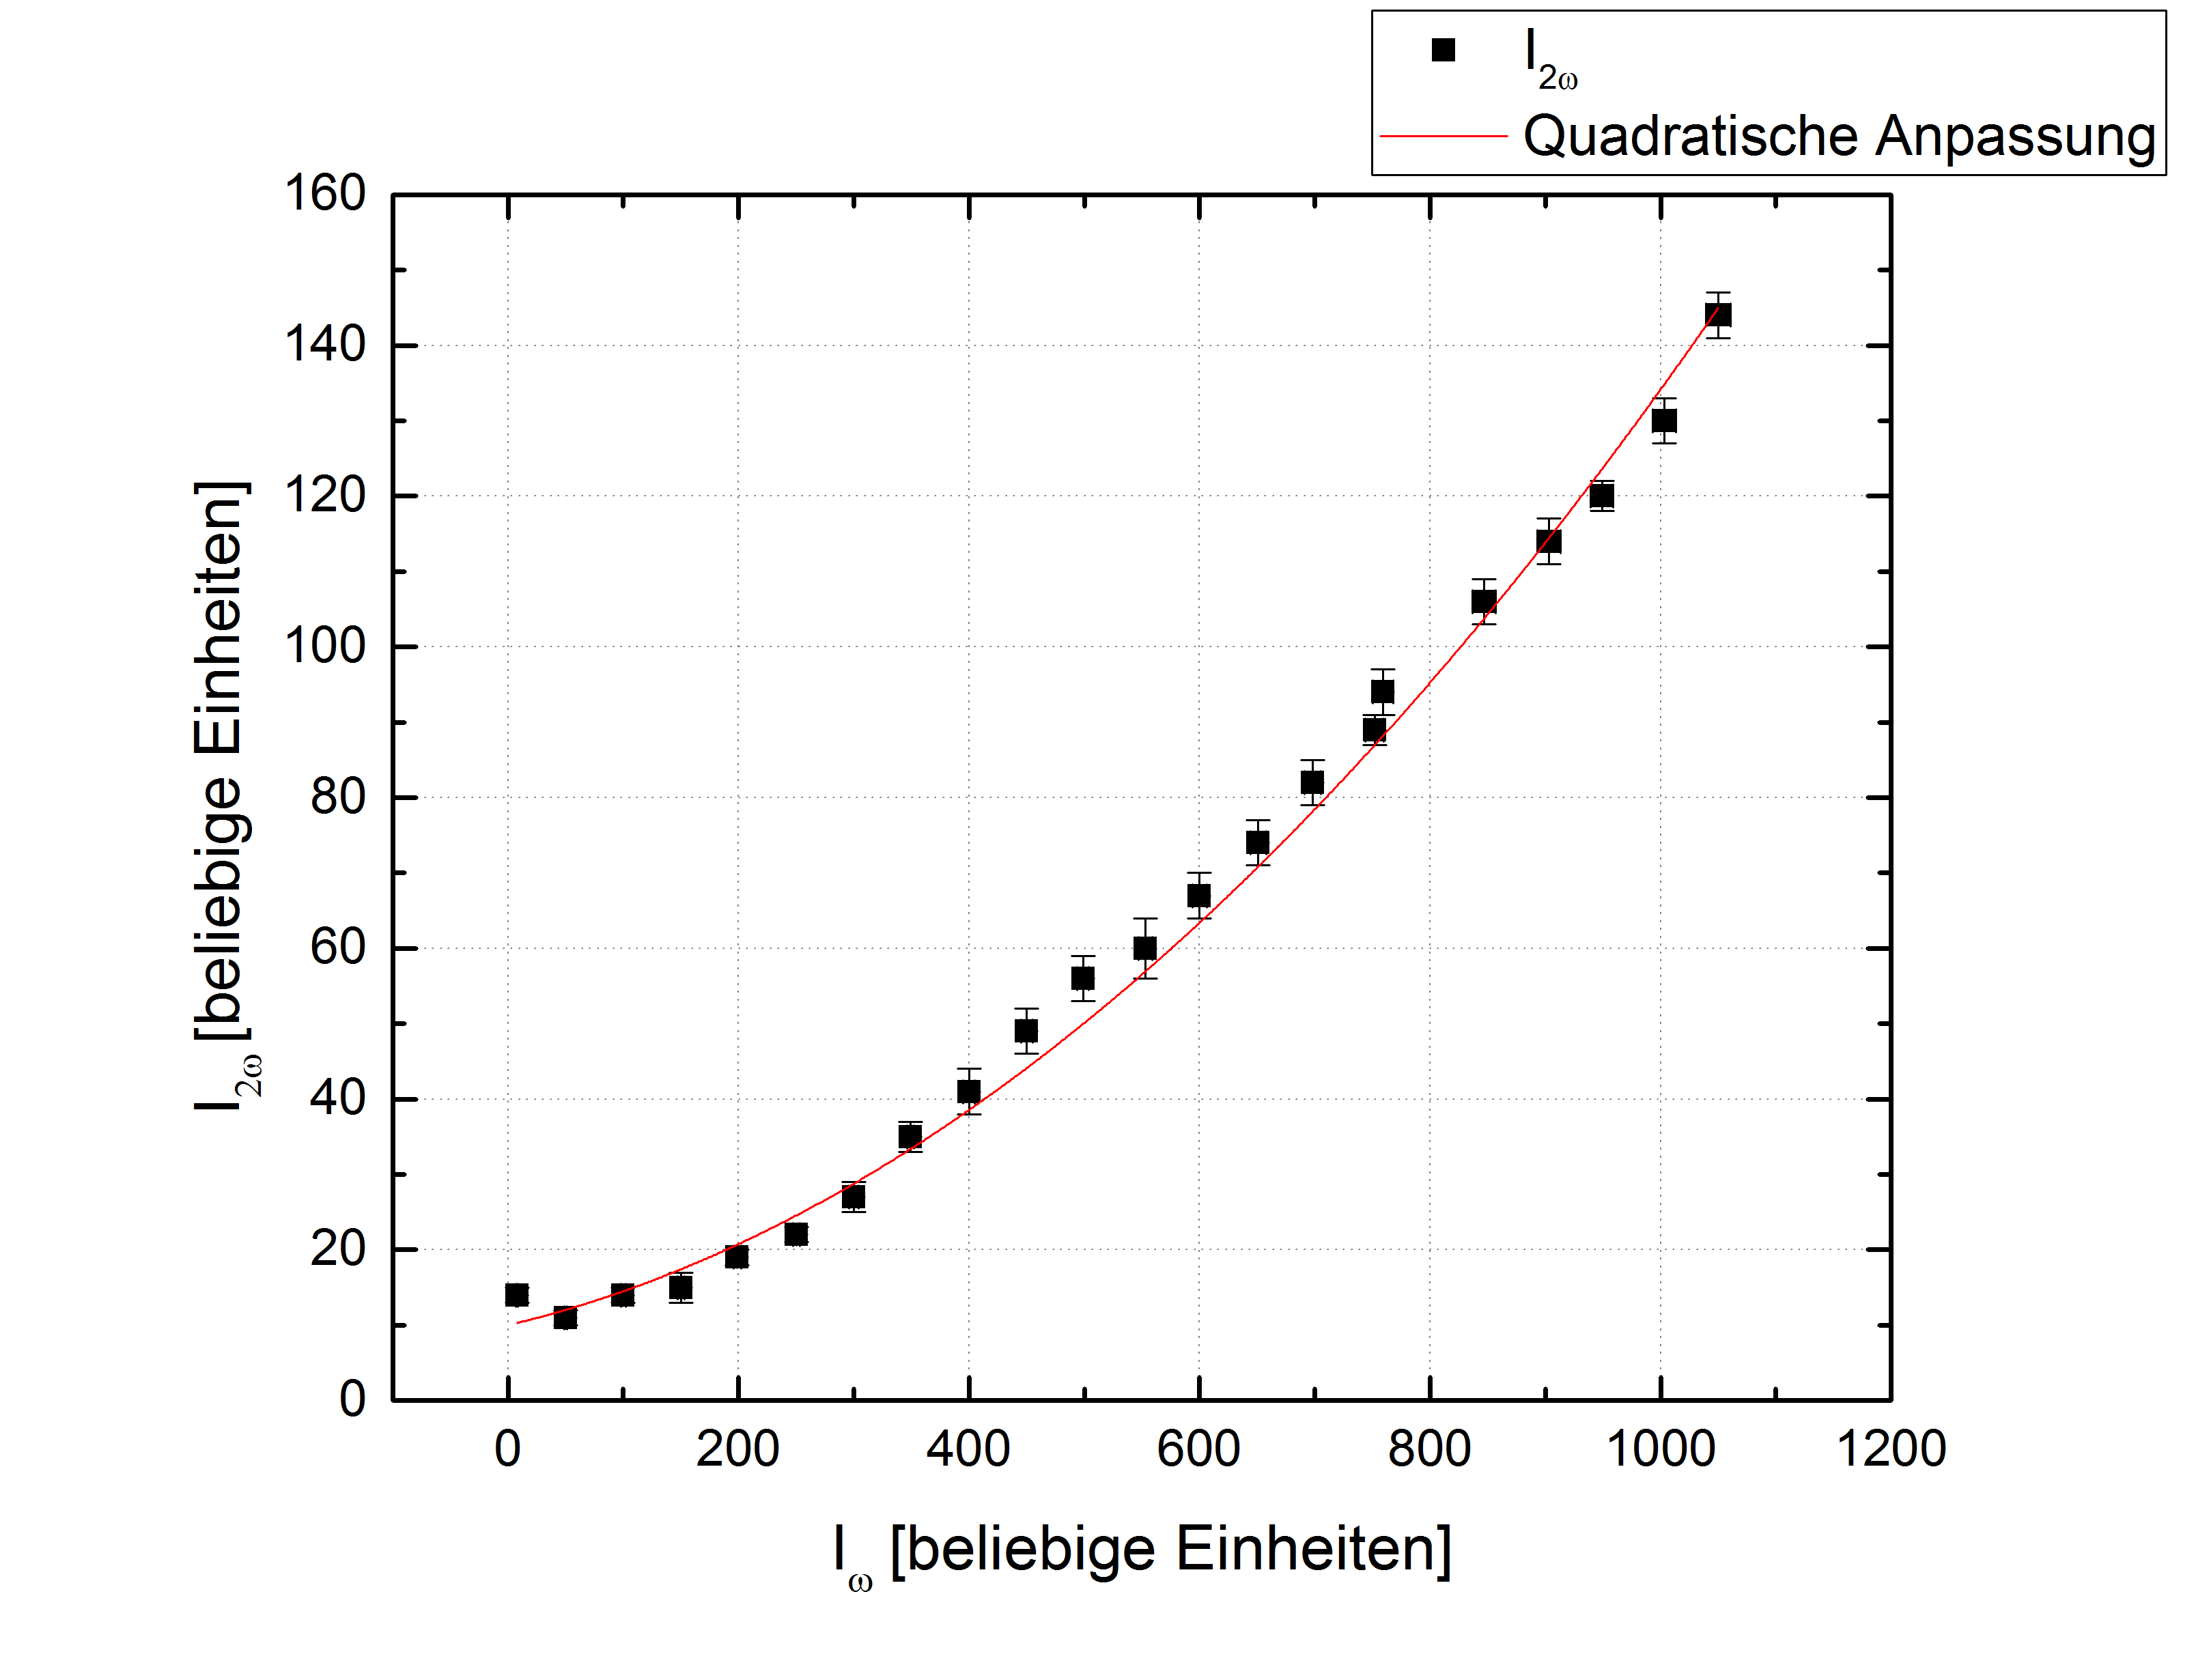
\includegraphics[scale=.5]{Bilder/IntPol2.png}
		\caption{Quadratische Anpassung der Intensitätsabhängigkeit}
		\label{pol2}
	\end{center}
\end{figure}

\subsection{Spektralanalyse der Laser}
Beim im Folgenden beschriebenen Versuchsteil wurden die Spektren der Laser mit Hilfe eines Spektrometers analysiert. Dieses Spektrometer muss jedoch zunächst kalibriert werden, was mit Hilfe eines Helium-Neon-Lasers erreicht wurde, der sich aufgrund seiner extrem schmalen Frequenzbreite gut dafür eignet. \newline
Das Spektrometer wurde dabei auf das doppelte, was nur dem hier voliegenden Versuchsaufbau geschuldet ist bekannte Wellenlänge des Lasers von 1266 nm eingestellt und ein Spektrum aufgenommen. Die zweite Messung wurde dann ebenfalls mit dem HeNe-Laser durchgeführt, allerdings wurde das Spektrometer hier auf 1286 nm gestellt, was eine Verschiebung der die Wellenlängen registrierenden Pixel hervorruft. In Abbildung \ref{1266nm} und \ref{1286nm} sind die zueinander verschobenen Linien des HeNe-Laserspektrums zu sehen.
\begin{figure}[H]
	\begin{center}
		\subfigure[1266 nm]{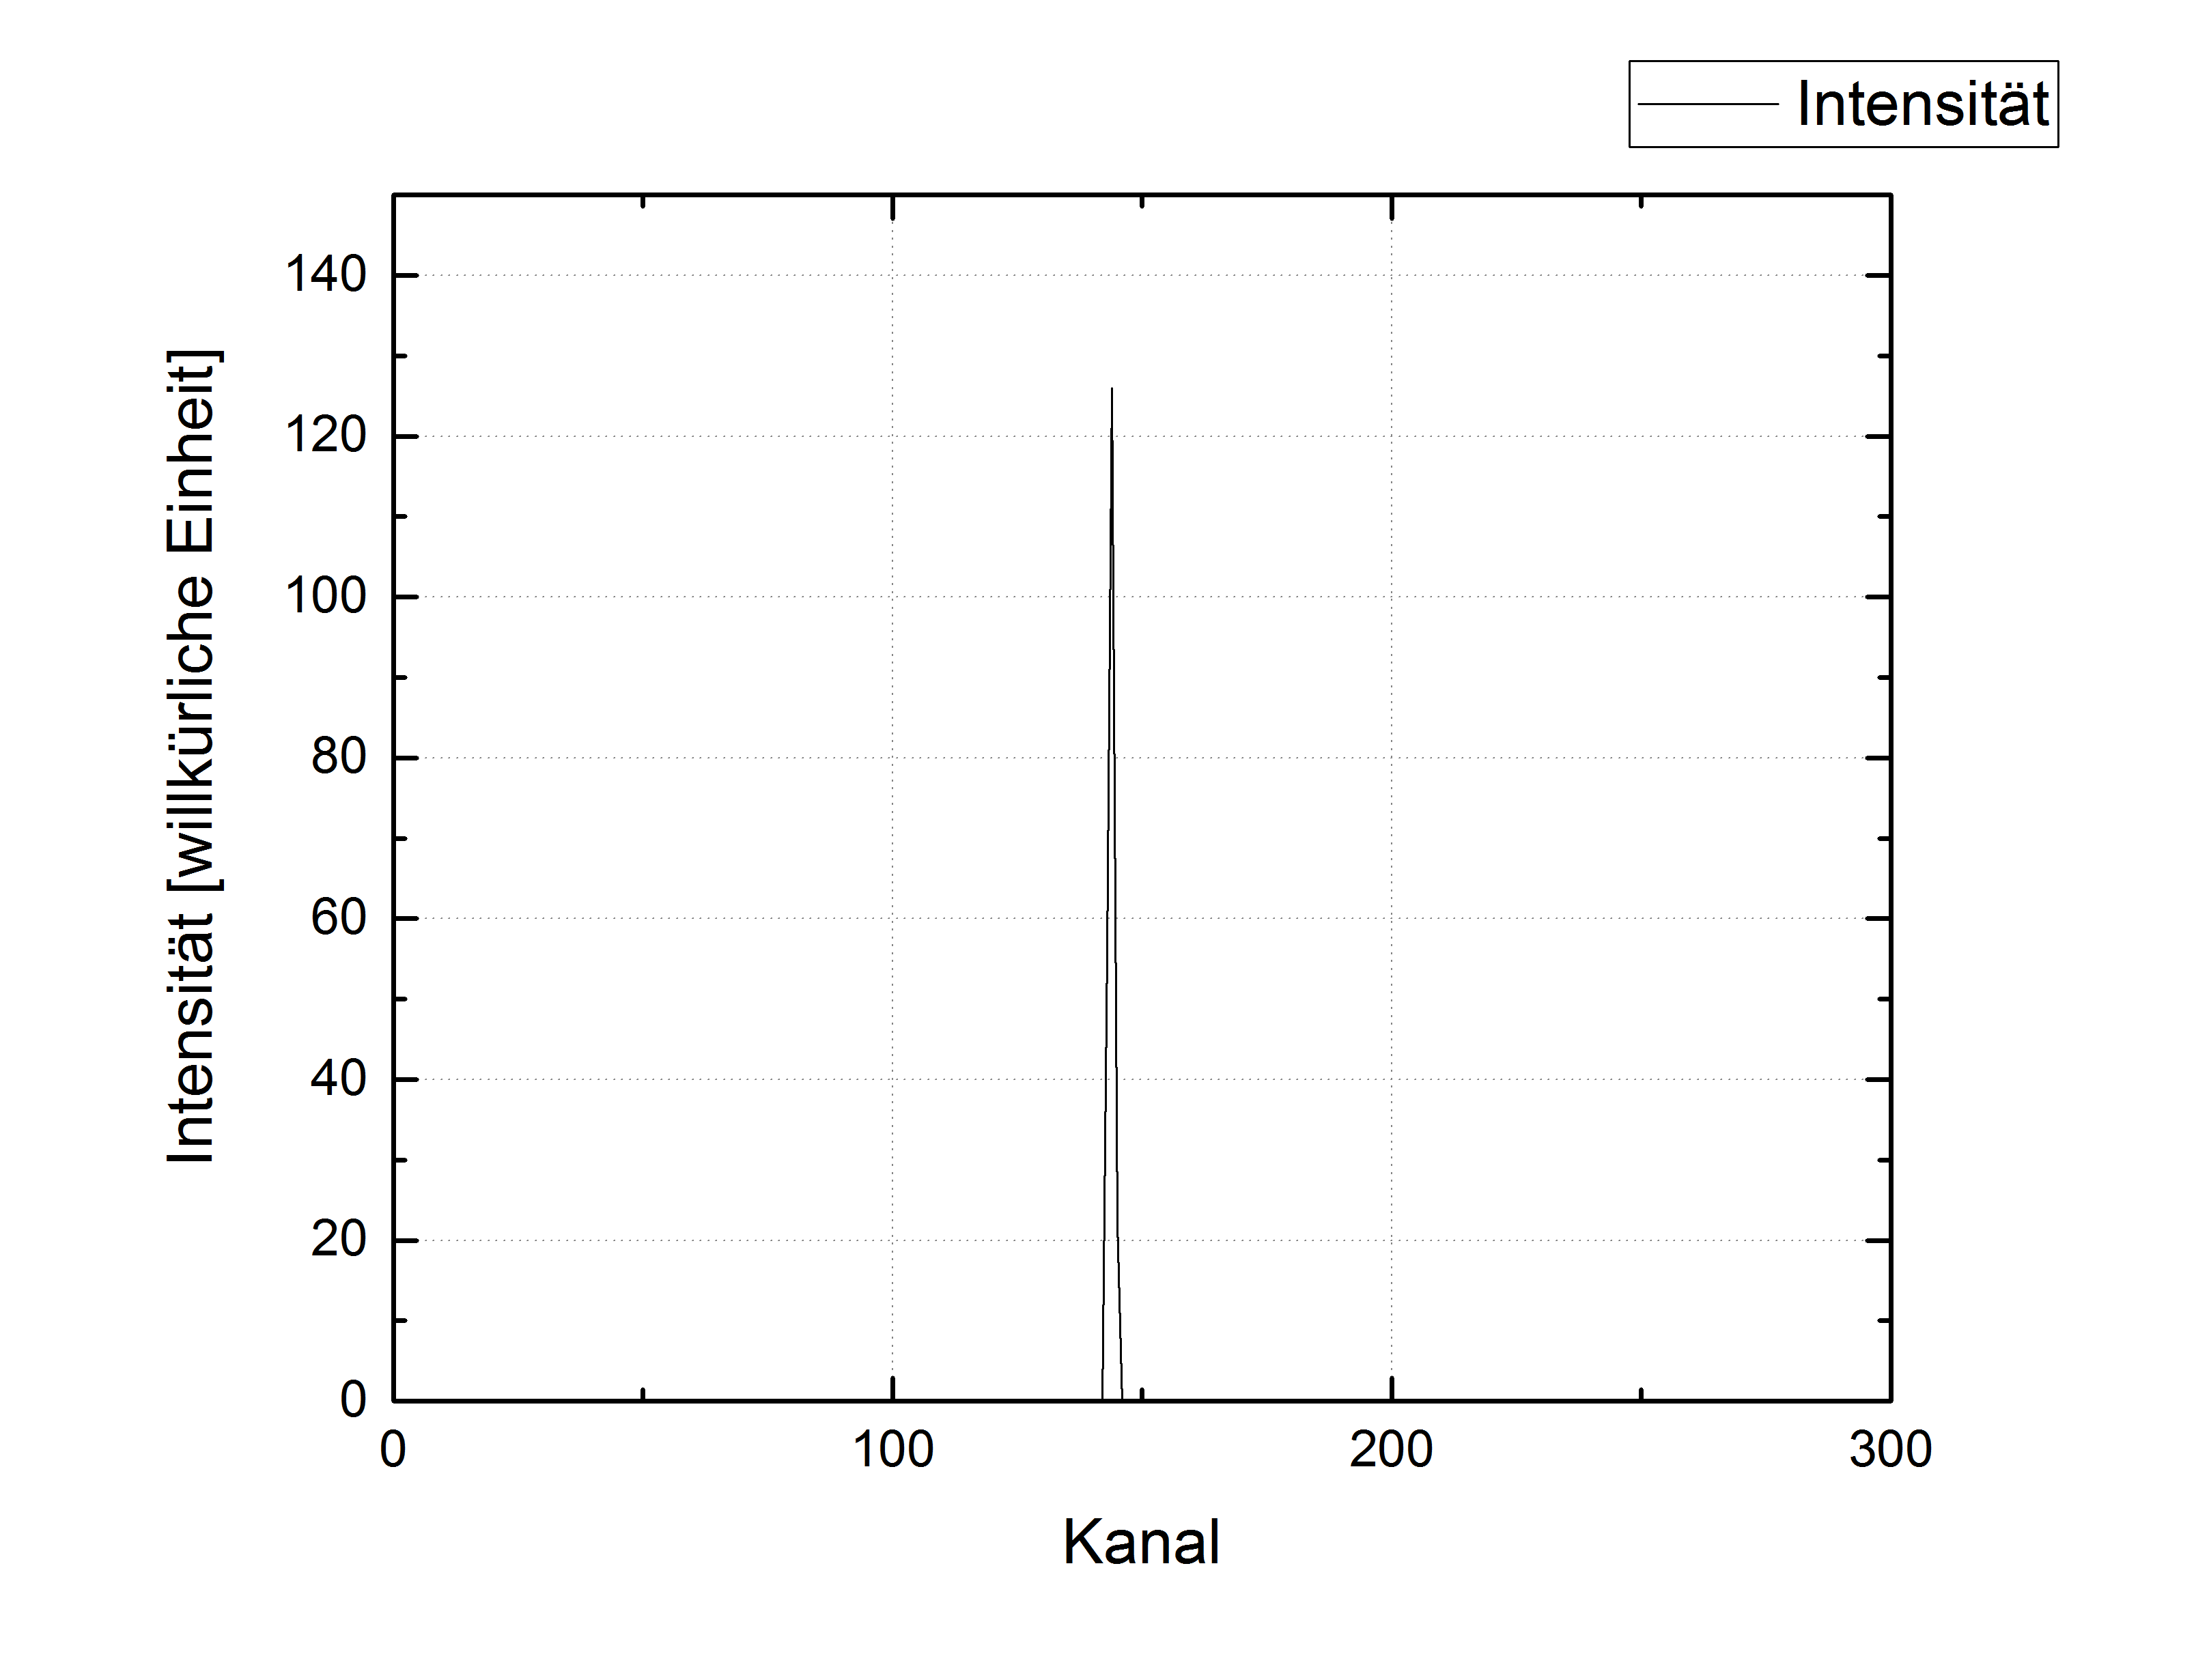
\includegraphics[scale=0.29]{Bilder/Kal1.png}\label{1266nm}}
		\subfigure[1286 nm]{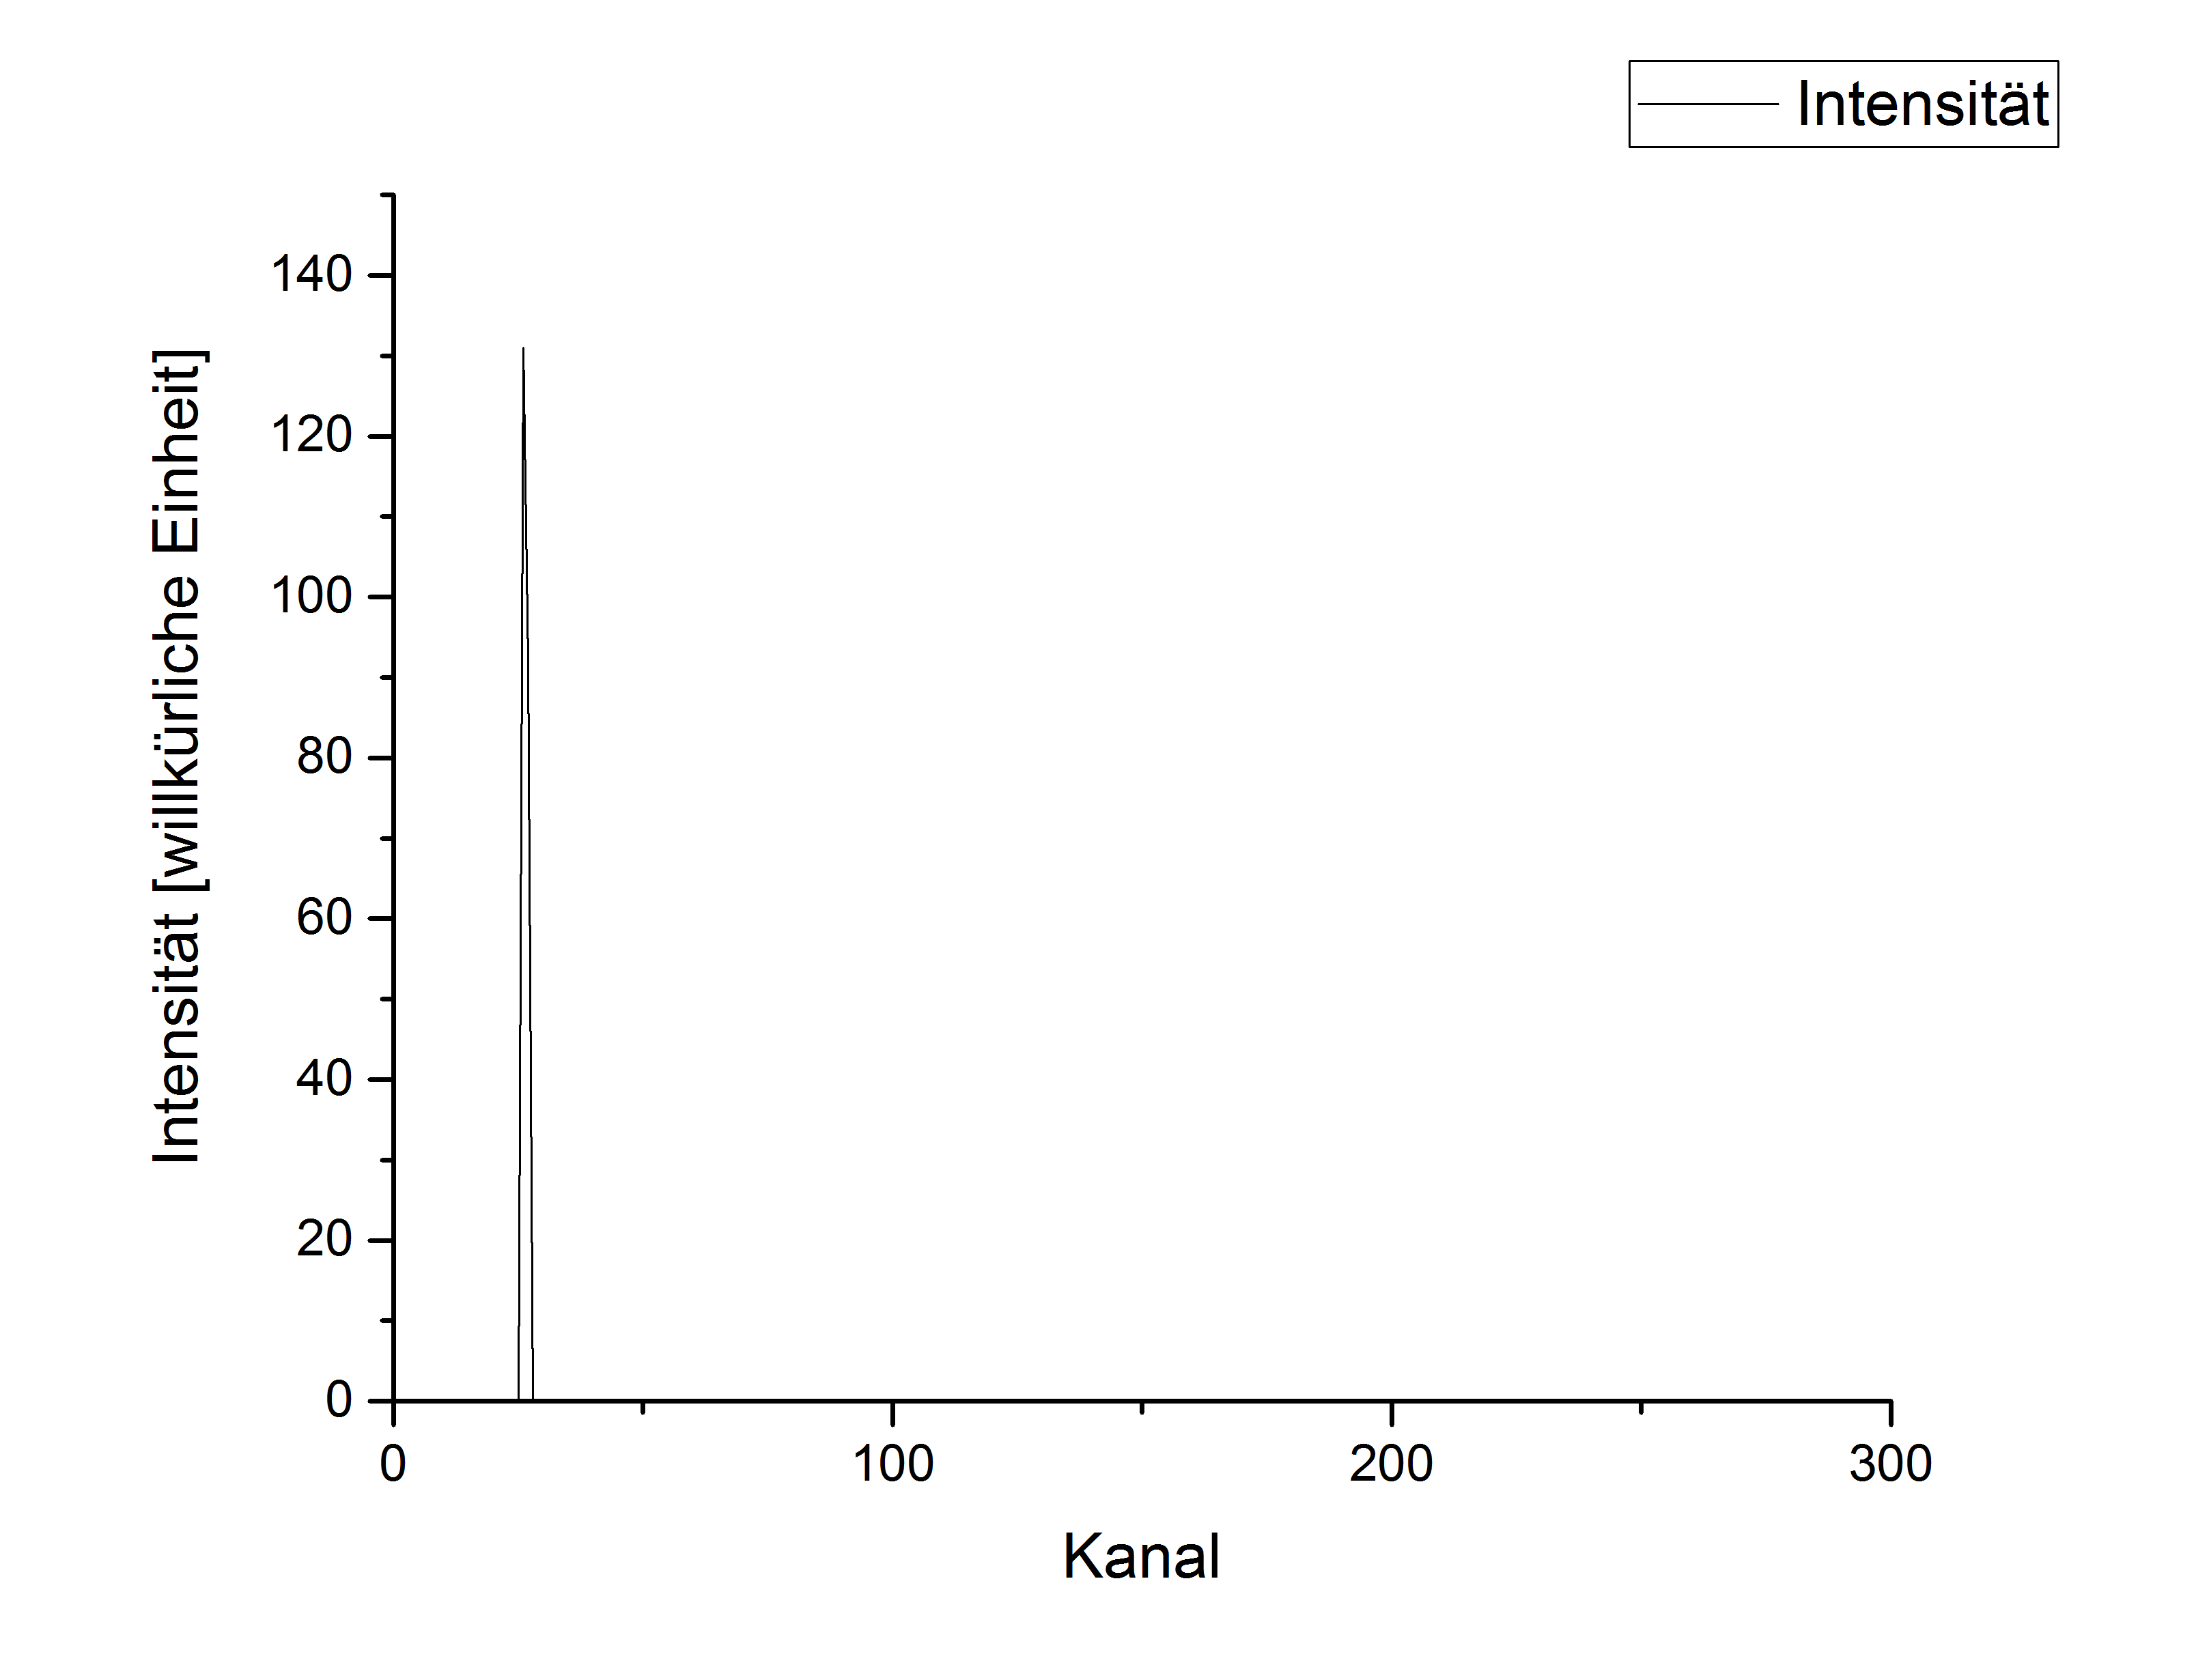
\includegraphics[scale=0.29]{Bilder/Kal2.png}\label{1286nm}}
		\label{kalib}
	\end{center}
\end{figure}
Um die scharfen Linien besser zu sehen wurden hier statt der üblichen Punktdiagramme Liniendiagramme verwendet. Man sieht deutlich wie schmal die Frequenzbreite für diesen Laser ist. Der Peak hat in Abbildung \ref{1266nm} eine Breite von drei Pixeln beziehungsweise zwei Pixeln in Abbildung \ref{1286nm}. Der Abstand der beiden Linien beträgt hier 118 Pixel, womit sich mit 
\begin{equation}
\triangle\lambda=\frac{10\text{nm}}{\triangle\text{Pixel}}=0.00847 \frac{\text{nm}}{\text{Pixel}}
\label{abstand}
\end{equation}
ergibt. Jeder Pixel deckt also einen Wellenlängenbereich von 0.00847 nm ab. Unter Berücksichtigung eines wellenlängenabhängigen Offsets des Spektrometers ergibt sich für die Wellenlänge in Abhängigkeit des aktivierten Pixels
\begin{equation}
\lambda=\frac{\lambda_{\text{set}}}{2}-\triangle\lambda(\text{Pixel}-256)+0.0189\left(\frac{\lambda_{\text{set}}}{2}-1064.36\text{nm}\right)
\label{wellenlänge}
\end{equation}
mit $\lambda_{\text{set}}$ der an dem Spektrometer eingestellten Wellenlänge. Zum Test dieser Formel und ob $\triangle\lambda$ richtig berechnet wurde wurde Gleichung \ref{wellenlänge} auf beide Graphen in Abbildung \ref{kalib} angewendet. Sind die bisherigen Ergebnisse korrekt müssen beide Linien aufeinanderfallen, da sie dem gleichen Spektrum bei anders eingestelltem Spektrometer und tatsächlich ergibt sich das Bild in \ref{test}
\begin{figure}[H]
	\begin{center}
		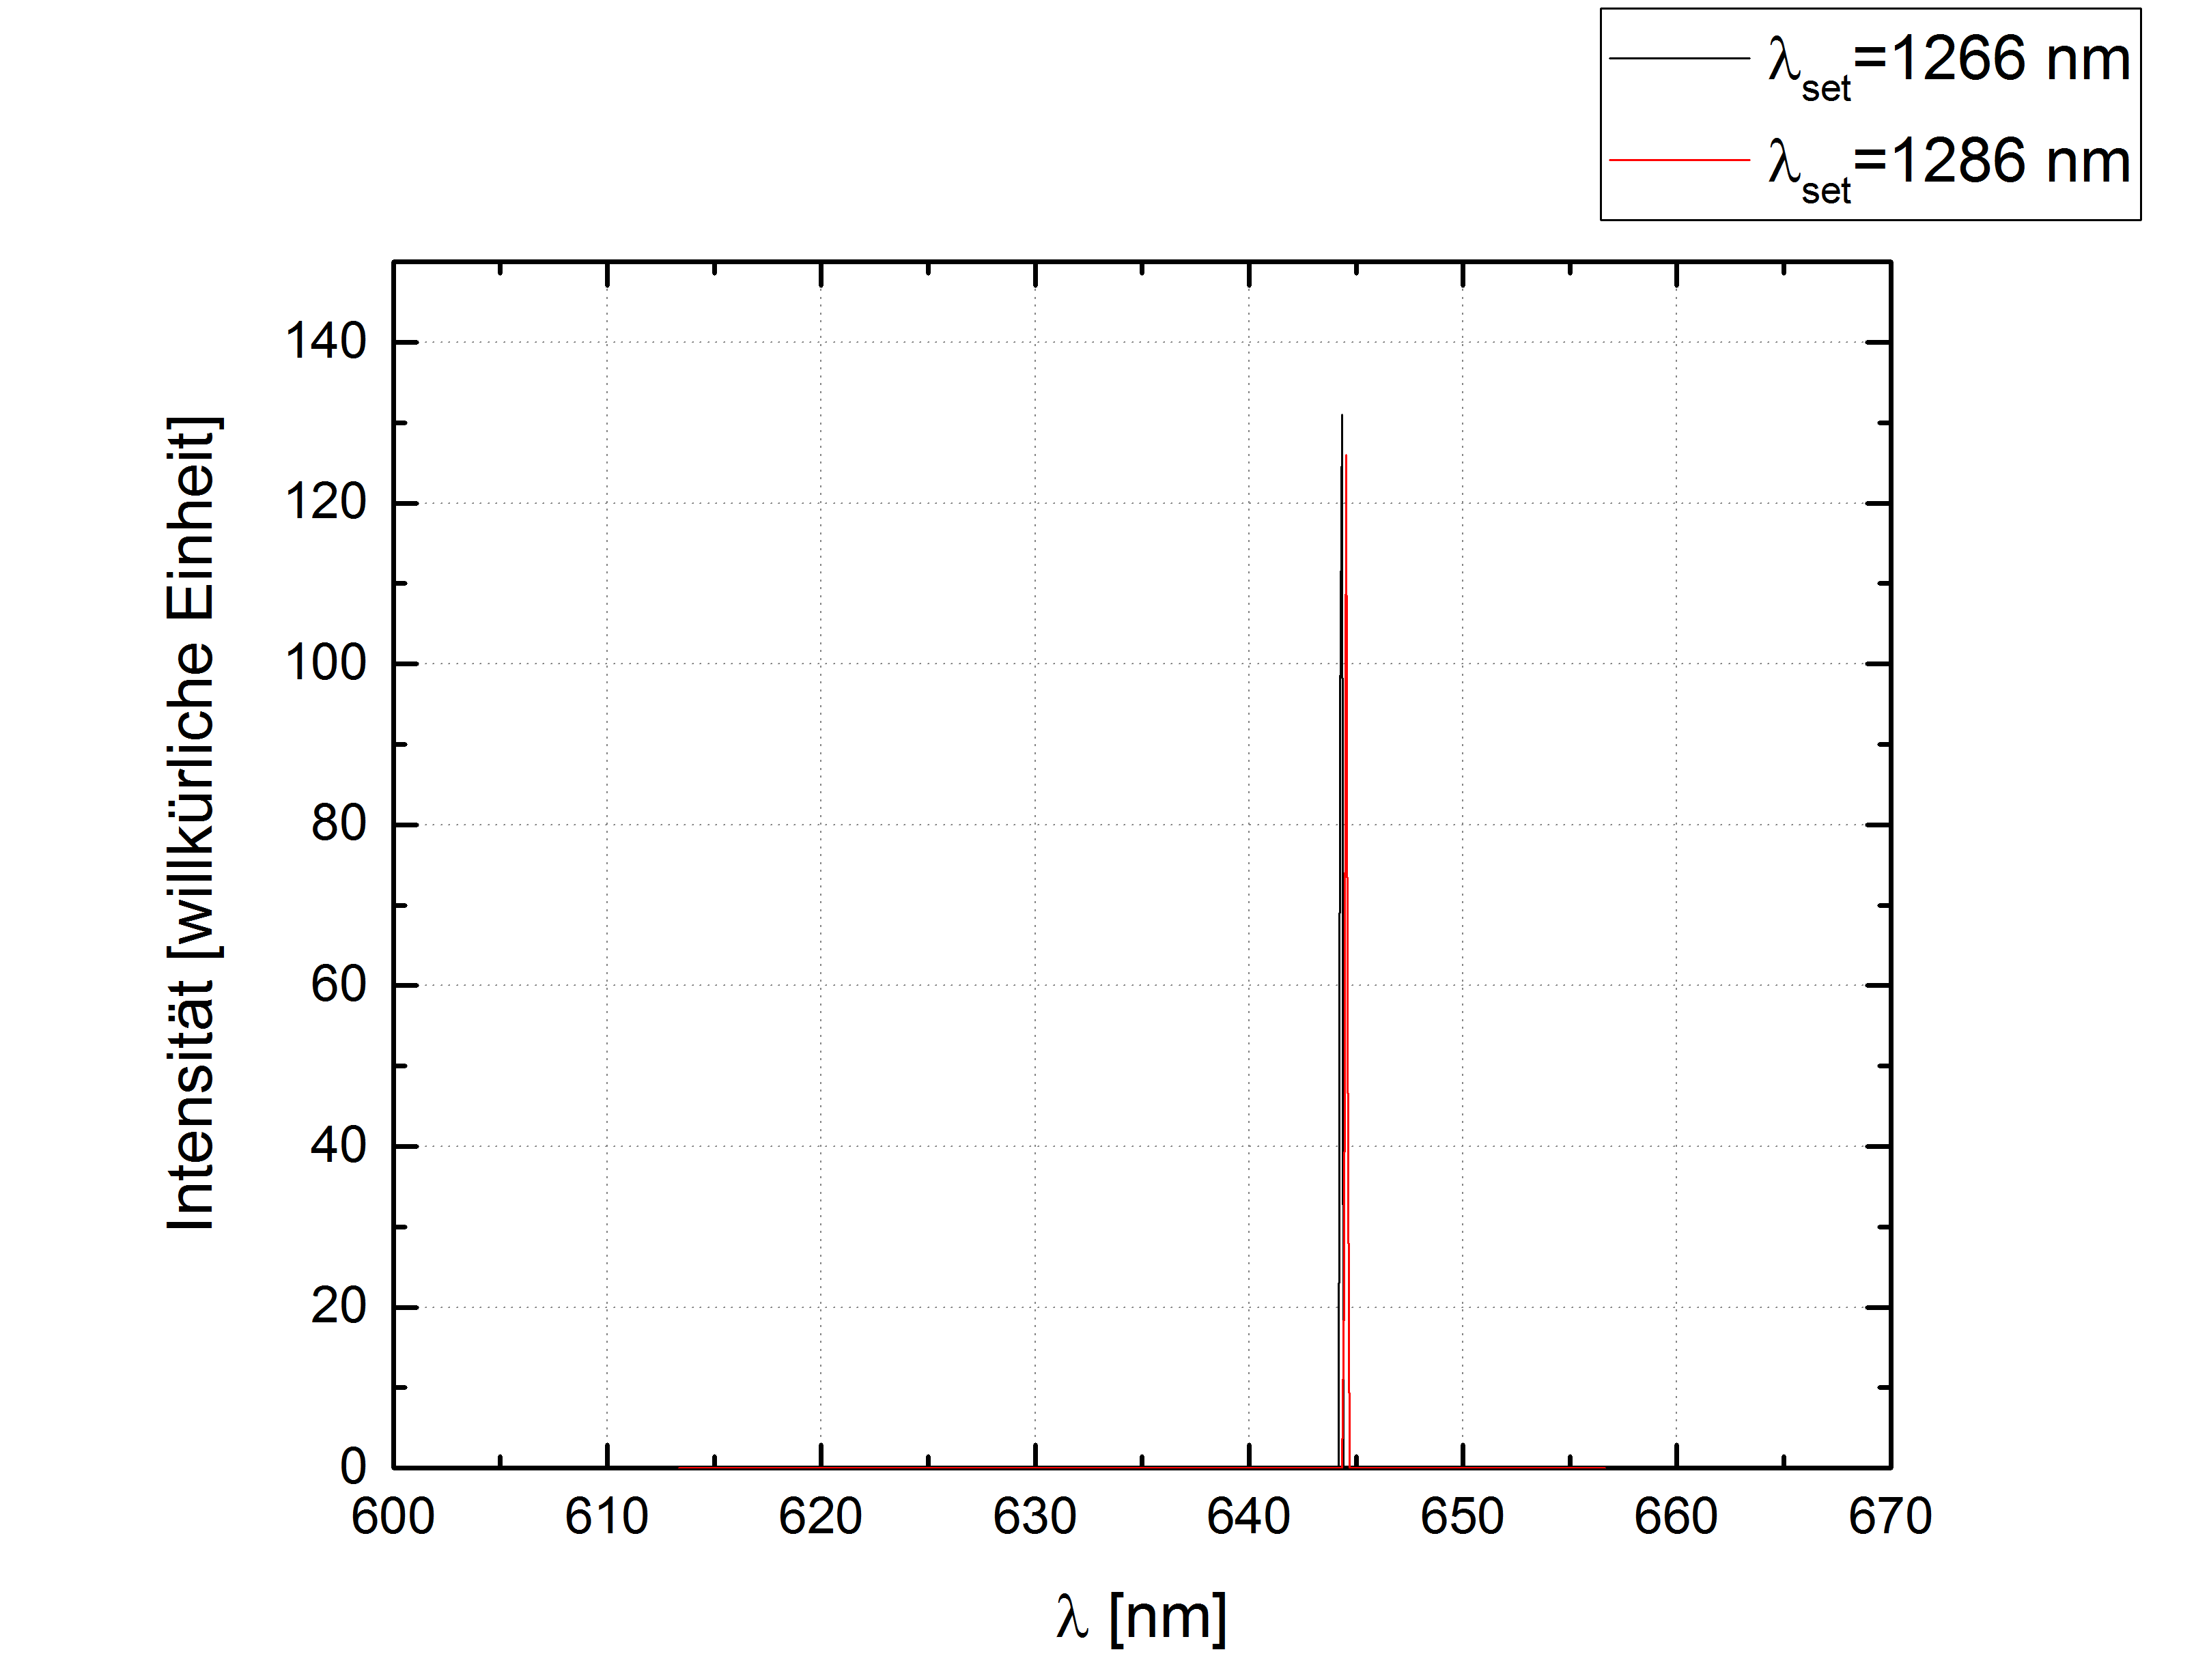
\includegraphics[scale=.5]{Bilder/Test.png}
		\caption{Überprüfung von Gleichung \ref{wellenlänge} und \ref{abstand}}
		\label{test}
	\end{center}
\end{figure}
Anzumerken ist, dass aus nicht näher zu bestimmenden Gründen die gemessene Wellenlänge um circa 10 nm gegenüber der eigentlichen Wellenlänge des Laserlichts verschoben ist. Diese Verschiebung ist auch bei den anderen aufgenommenen Spektren zu beobachten, beträgt dort jedoch nur 2-3 nm. Da für die weiteren Betrachtungen die genaue Wellenlänge des Peaks nicht von großer Bedeutung ist, sondern nur dessen Breite, auf die die Verschiebung keine Auswirkung hat, wird diese nicht weiter berücksichtigt.\newline
Nach dieser Kalibrierung wurde das Spektrometer auf 1590 nm eingestellt, was der tatsächlichen Wellenlänge der Pumpdiode von 795 nm entspricht. \newline
In Abbildung \ref{spek1} ist das Spektrum der Laserdiode für die in \ref{diode} angesprochenen verschiedenen Leistungsbereiche der Laserdiode. Wie bereits erwähnt entspricht Abbildung \ref{kennpump} im Bereich \newline < 8 A nicht der Wahrheit. Wie in Abbildung \ref{flour} zu sehen ist wird auch für geringe Stromstärken Licht emmitiert. Diese Emission beruht allerdings auf spontaner und nicht auf der für Laser benötigten stimulierten Emission, weshalb dieser Bereich auch Floureszenzbereich genannt wird. Aus diesem Grund weißt man auch ein weitaus breiteres Spektrum nach als man es für einen Laser erwarten würde. Außerdem ist zu bemerken, die gemessene Intensität um einen Faktor 4-5 niedriger ist als im Übergangs - oder Laserbereich, was erklärt, warum in Abbildung \ref{kennpump} für diese Stromstärken kein Licht nachgewiesen wurde, es wurde schlicht von den vor dem Detektor angebrachten Filten komplett unterdrückt. \newline 
In Abbildung \ref{ueb} ist der so genannte Übergangsbereich zu sehen, welcher in Abbildung \ref{kennpump} von dem langsamen Anstieg der gemessenen Intensität beschrieben wird. In dem Spektrum selbst ist immer noch ein breiter, auf Floureszenz beruhender Anteil zu sehen, in dessen Mitte sich jedoch bereits ein sehr schmaler und intensiverer Peak ausbildet, der auf einen allmählichen Beginn der Lasertätigket zurückzuführen ist.
\begin{figure}[H]
	\begin{center}
		
		\subfigure[Floureszenzbereich]{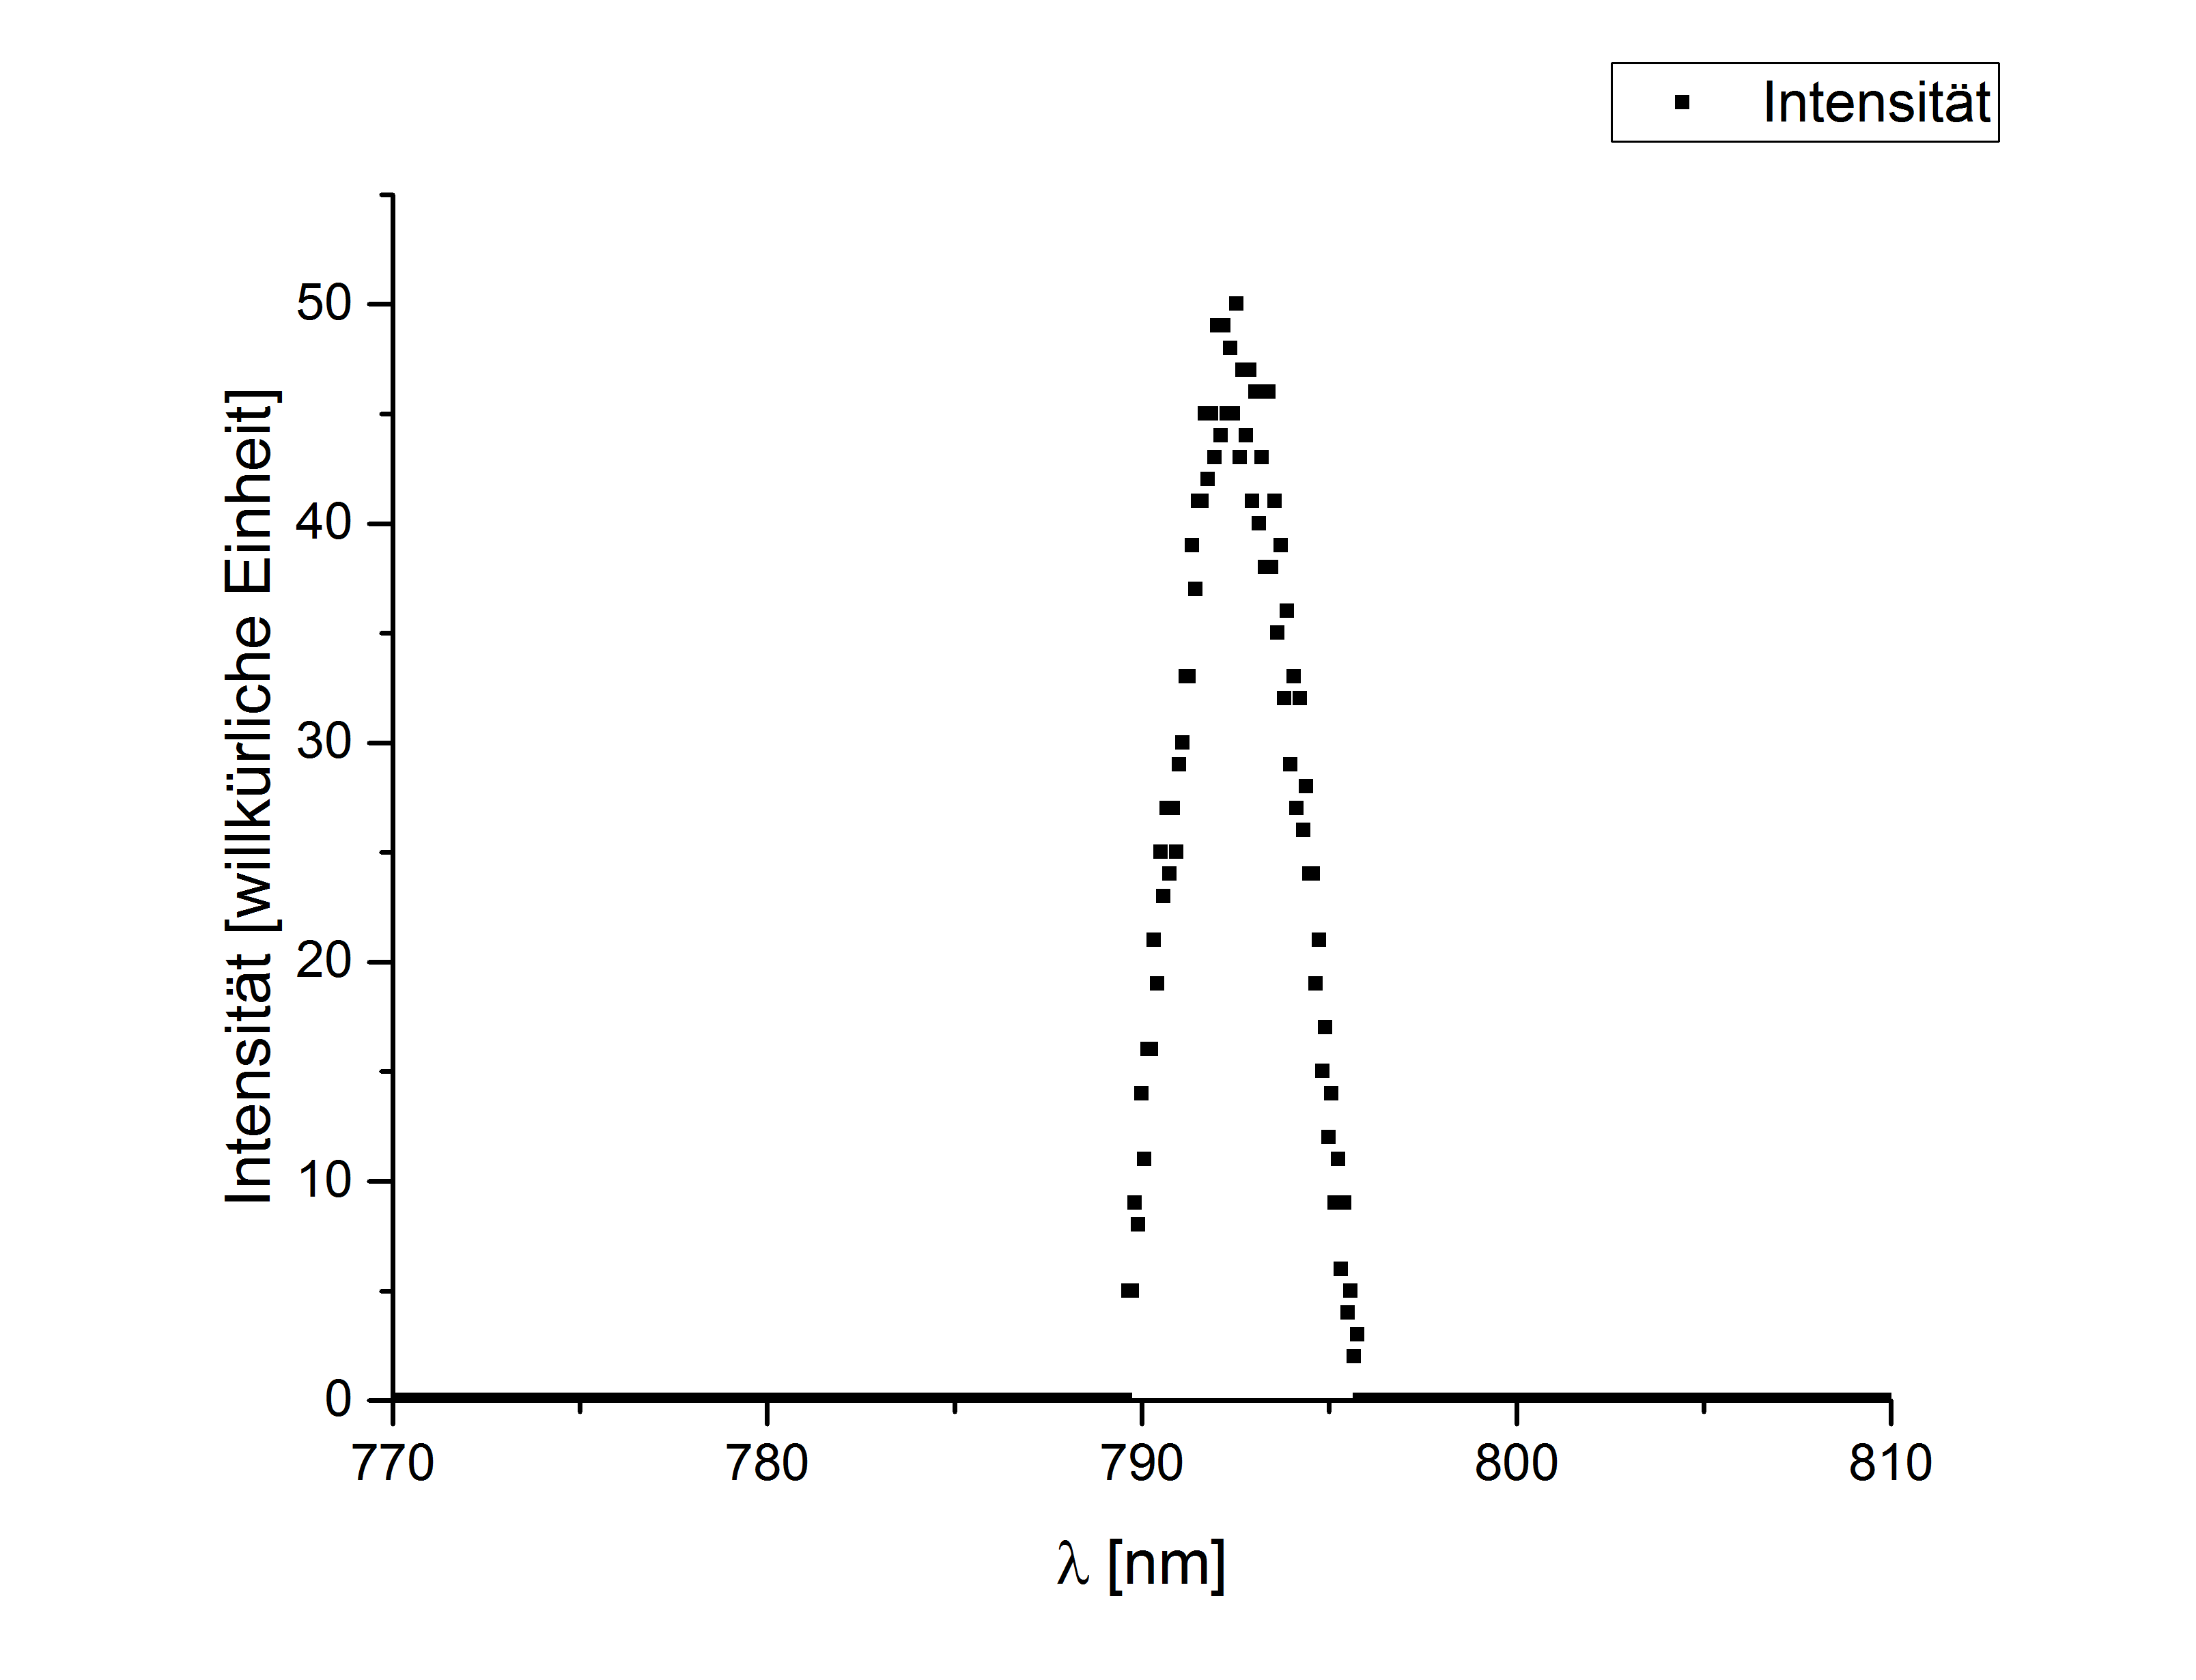
\includegraphics[scale=.29]{Bilder/Floureszenz.png}\label{flour}}
		\subfigure[Übergangsbereich]{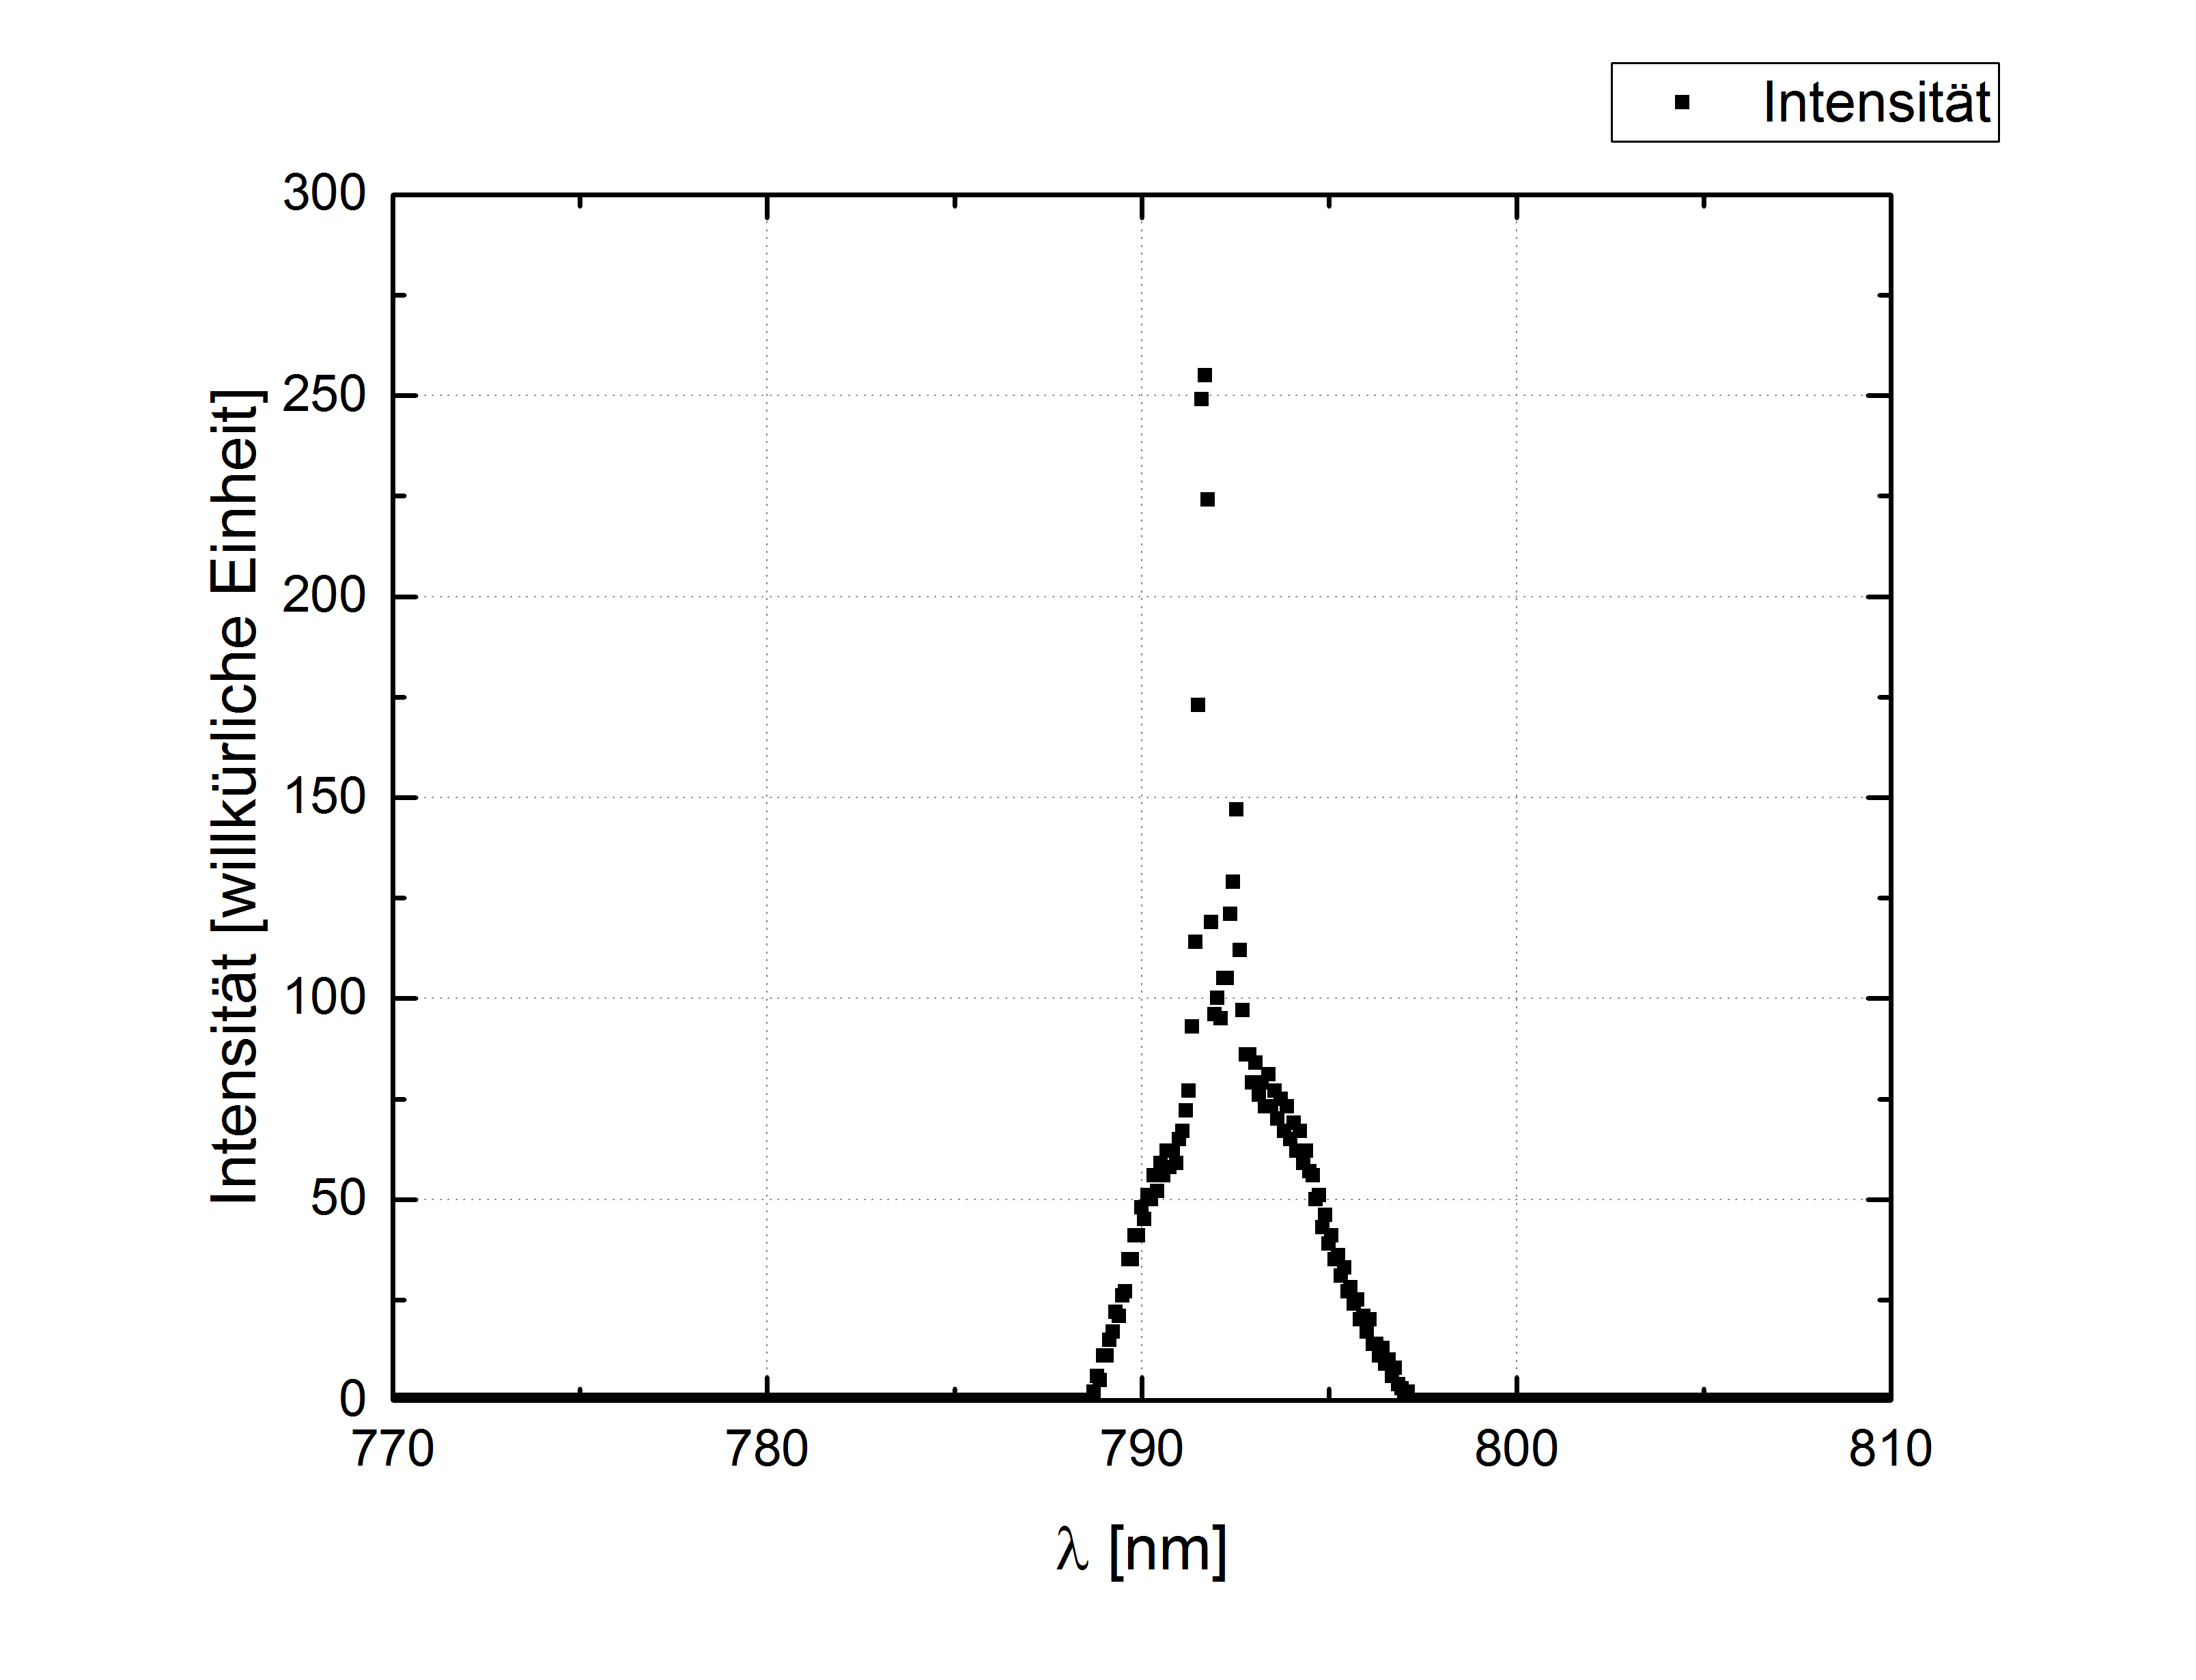
\includegraphics[scale=.29]{Bilder/Uebergang.png}\label{ueb}}
		\subfigure[Laserbereich]{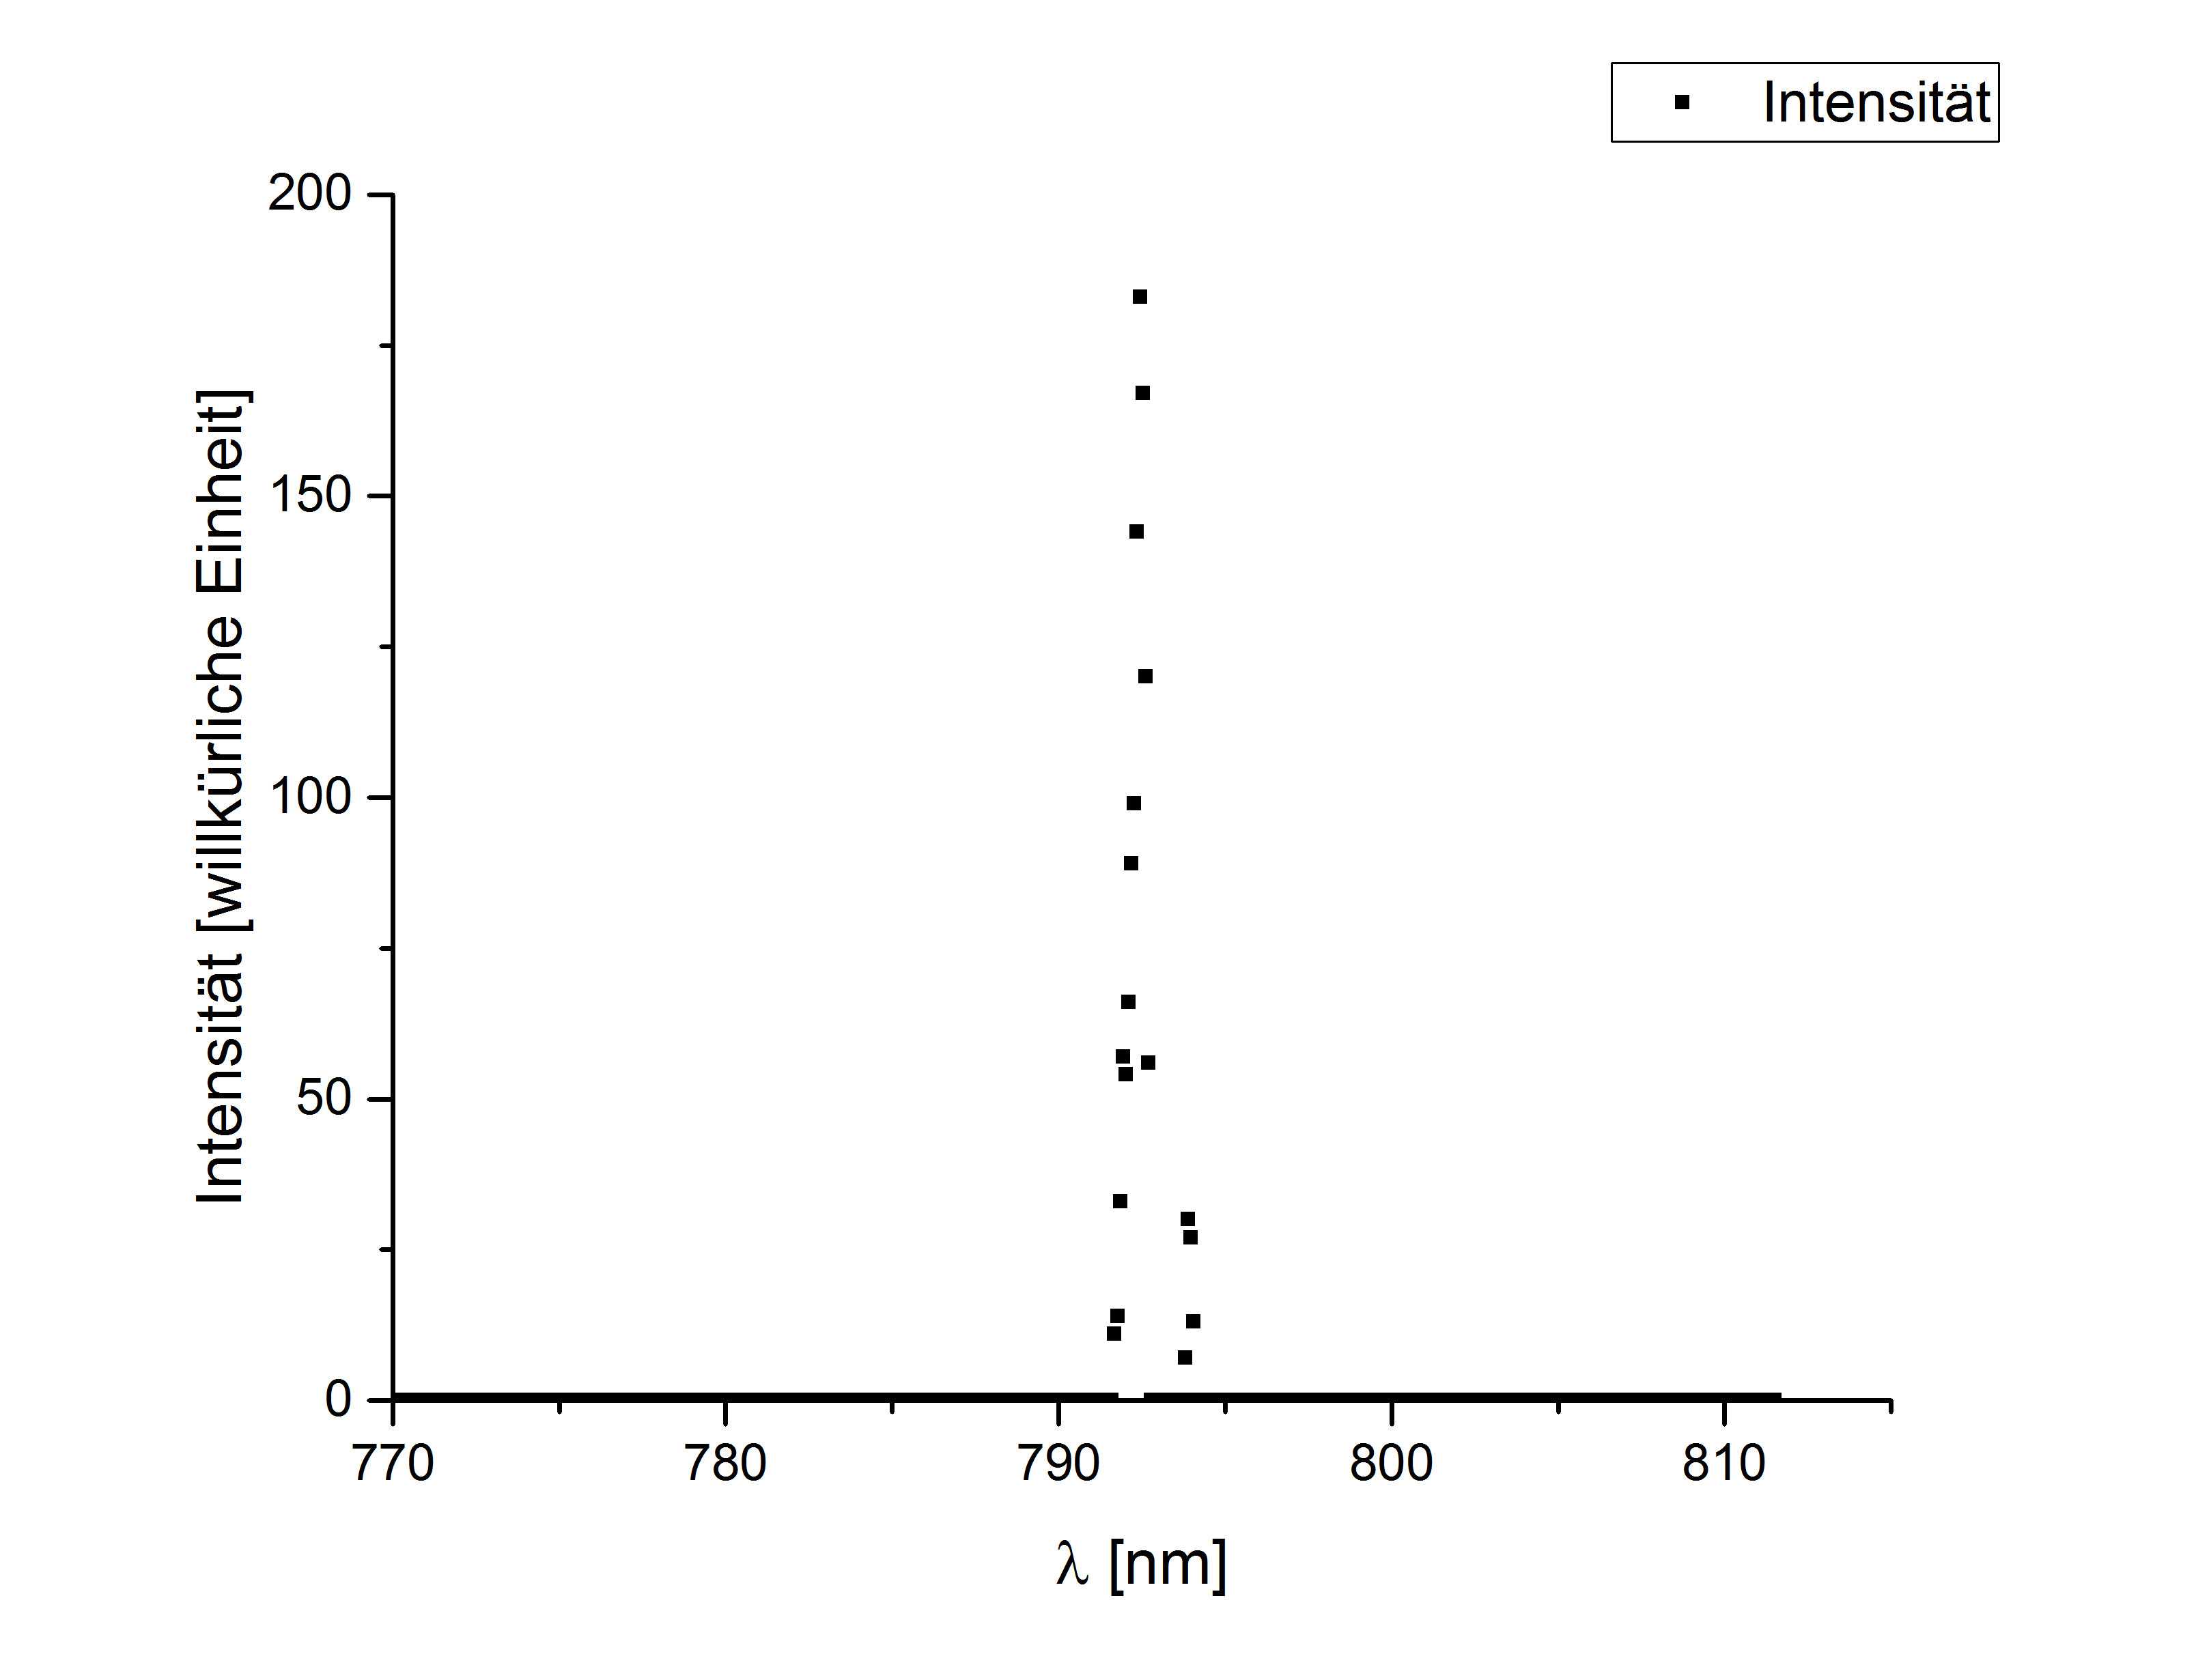
\includegraphics[scale=.29]{Bilder/Laser.png}\label{laser}}
		\caption{Spektrum der Pumpdiode für verschiedene Leistungsbereiche}
		\label{spek1}
	\end{center}
\end{figure}
In Abbildung \ref{laser} schließlich ist ein sehr hoher und schmaler Peak zu sehen, der darauf hinweißt, dass die Lasertätigkeit in der Laserdiode voll aufgenommen wurde. Anzumerken ist hier jedoch, dass sich dieser im unteren Bereich verbreitert, was vor allem im Vergleich mit \ref{flour} durch die stets vorhande Floureszenz und damit spontane Emission von Licht in der Diode erklären lässt. Bei der Höhe des Laserpeaks jedoch ist dies jedoch ein nahezu vernachlässigbarer Effekt. \newline
Als letztes wurde das Spektrum des Nd:YLF-Lasers gemessen, welches in  Abbildung \ref{lasery} zu sehen ist
\begin{figure}[H]
	\begin{center}
		\includegraphics[scale=.5]{Bilder/Lasery.png}
		\caption{Spektrum des Nd:YLF-Lasers}
		\label{lasery}
	\end{center}
\end{figure}
Man erkennt deutlich einen schmalen, intensiven Peak, wie man ihn für einen Laser erwartet. Wie bereits erwähnt interessiert man sich nun für die Bandbreite dieses Lasers. Die gemessene Breite $\delta_m$ des Lasers ist dabei nicht direkt die reale Breite des Spektrums $\delta_r$, sondern hängt mit dem Auflösungsvermögen $\delta$ des Spektrometers wie folgt zusammen
\begin{equation}
\delta_r=\sqrt{\delta_m^2-\delta^2}
\label{breite}
\end{equation}
Nun kann für diesen Versuch angenommen werden, dass die Auflösung des Spektrometers gleich der Bandbreite des HeNe-Spektrums ist, denn es gilt
\begin{equation}
\delta=\sqrt{\delta_m^2-\delta_r^2}
\label{beweis}
\end{equation}
Nun gilt für den Zusammenhang zwischen Frequenzbreite und Wellenlängenbreite des Pulses
\begin{equation}
\triangle\lambda=\lambda_1-\lambda_2=\frac{c}{f_1}-\frac{c}{f_2}\Rightarrow \triangle f=f_1-f_2=\frac{\triangle\lambda-f_1f_2}{c}=\triangle\lambda\:\frac{c}{\lambda_1\lambda2}
\label{umrechnung}
\end{equation}
Mit $\lambda_1$ und $\lambda_2$ den Wellenlängen bei der halben Höhe des Maximiums beziehungsweise $\lambda_{1,2}=\lambda_{\text{max}}\pm\sigma$ mit $\lambda_{\text{max}}$ der Wellenlänge am Maximum und $\sigma$ der Halbwertsbreite. Anlegen von Gaußkurven an die beiden Graphen in Abbildung \ref{test} ergibt Halbwertsbreiten von 0.044 nm beziehungweise 0.124 nm. Nach Gleichung (\ref{umrechnung}) ergibt sich so ein Mittelwert von $\triangle f=62.98$ Hz = $\delta_m$. Nun beträgt die reale Halbwertsbreite des HeNe-Lasers maximal 10$^{-3}$nm, was einer Frequenzdifferenz von $\delta_r=$ 0.75Hz $\approx0.01\delta_m$ entspricht. Eingesetzt in Gleichung (\ref{beweis}) ergibt sich somit
\begin{equation*}
\delta=\sqrt{\delta_m^2-\delta_r^2}\approx\sqrt{\delta_m^2-(0.01\delta_m)^2}=\sqrt{\delta_m^2-0.0001\delta_m^2}\approx\sqrt{\delta_m^2}=\delta_m
\end{equation*}
Man sieht also, dass in diesem Fall das Auflösungsvermögen des Spektrometers in guter Näherung der gemessenen Halbwertsbreite des HeNe-Lasers entspricht. Um nun die Breite des Nd:YLF-Lasers zu messen muss zunächst die Halbwertsbreite der gemessenen Werte bestimmt werden, was wiederum mit einer Gaußfunktion erreicht wird. Somit ergibt sich eine Halbwertsbreite von 0.59 nm und so nach Gleichung (\ref{umrechnung}) eine Frequenzbreite von 160.76 Hz und somit nach (\ref{breite}) eine reale Frequenzbreite von 147.91 Hz.\newline
Als letzes lässt sich nun zusammen mit Hilfe der aus der Autokorrelation bestimmten Impulsdauer das Impulsdauer-Bandbreite-Produkt bestimmen, das ein Maß für die Güte eines Laserpulses darstellt und es gilt
\begin{equation}
\delta_r\cdot\tau=5.09\cdot10^{-12}\ll 0.441
\end{equation}